\documentclass[../thesis/thesis.tex]{subfiles}
\begin{document}
 \chapter{Prototype Design}

% Intro
% Introduce MLX

As discussed in the Literature Review, using an \iar appear to be the most viable way to achieve the high-level goals of this project. Thermosense \cite{beltran2013thermosense}, the primary occupancy sensor in the \iar space, used the low-cost Panasonic \geye sensor for this task. This sensor, costing around \$30USD, appears to be a prime candidate for use in this project, as it satisfied low-cost criteria, as well as being proven by Thermosense to be effective in this space. However, while still available for sale in the United States, we were unable to order the sensor for shipping to Australia due to export restrictions outside of our control. While such restrictions would be circumventable with sufficient effort, using a sensor with such restrictions in place goes against an implicit criteria of the parts used in the project being relatively easy to acquire.

This forced us to search for alternative sensors in the space that fulfill similar criteria but were more broadly available. The sensor we settled on was the \mlx \cite{MLXDatasheet}, an \iar with similar overall qualities that differed in several important ways; it provides a $16 \times 4$ grid of thermal information, it has an overall narrower field of view and it sells for approximately \$80USD. Like the \geye, the \mlx sensor communicates over the 2-wire \iic bus, a low-level bi-directional communication bus widely used and supported in embedded systems.

In an idealized version of this occupancy system, much like Thermosense this system would include wireless networking and a very small form factor. However, due to time and resource constraints, the scope of this project has been limited to a minimum viable implementation. Appendix \Fref{chap:architecture} discusses in detail how the introduction of new open standards in the Wireless Personal Area Network space could be used in future systems to provide robust, decentralized networking of future occupancy sensors. This prototype architecture has been designed such that a clear path to the idea system architecture discussed therein is available.


\section{Hardware}

\begin{table}
\centering
\begin{tabular}{|r|l|}
\hline
\textbf{Analysis Tier} & Raspberry Pi B+ \\ \hline
\textbf{Preprocessing Tier} & \ard Uno R3 \\ \hline
\textbf{Sensing Tier} & \acl{mlx} \& PIR \\ \hline
\end{tabular}
\caption{Hardware tiers}
\label{tab:sensor:tiers}
\end{table}

As reliability and future extensibility are core concerns of the project, a three-tiered system is employed with regards to the hardware involved in the system (\Fref{tab:sensor:tiers}). At the bottom, the Sensing Tier, we have the raw sensor, the \mlx, which communicate over \iic. Connected to these devices via those respective protocols is the Preprocessing Tier, run an embedded system. The embedded device polls the data from these sensors, performs necessary calculations to turn raw information into suitable data, and communicates this via Serial over USB to the third tier. The third tier, the Analysis Tier, is run on a fully fledged computer. In our prototype, it captures and stores both video data, and the Temperature and Motion data it receives over Serial over USB.

While at a glance this system may seem overly complicated, it ensures that a sensible upgrade path to a more feature-rich sensing system is available. In the current prototype, the Analysis Tier merely stores captured data for offline analysis, in future prototypes this analysis can be done live and served to interested parties over a RESTful API. In the current prototype, the Analysis and Sensing Tiers are connected by Serial over USB, in future prototypes, this can be replaced by a wireless mesh network, with many Preprocessing/Sensing Tier nodes communicating with one Analysis Tier node.

\begin{figure}
\centering
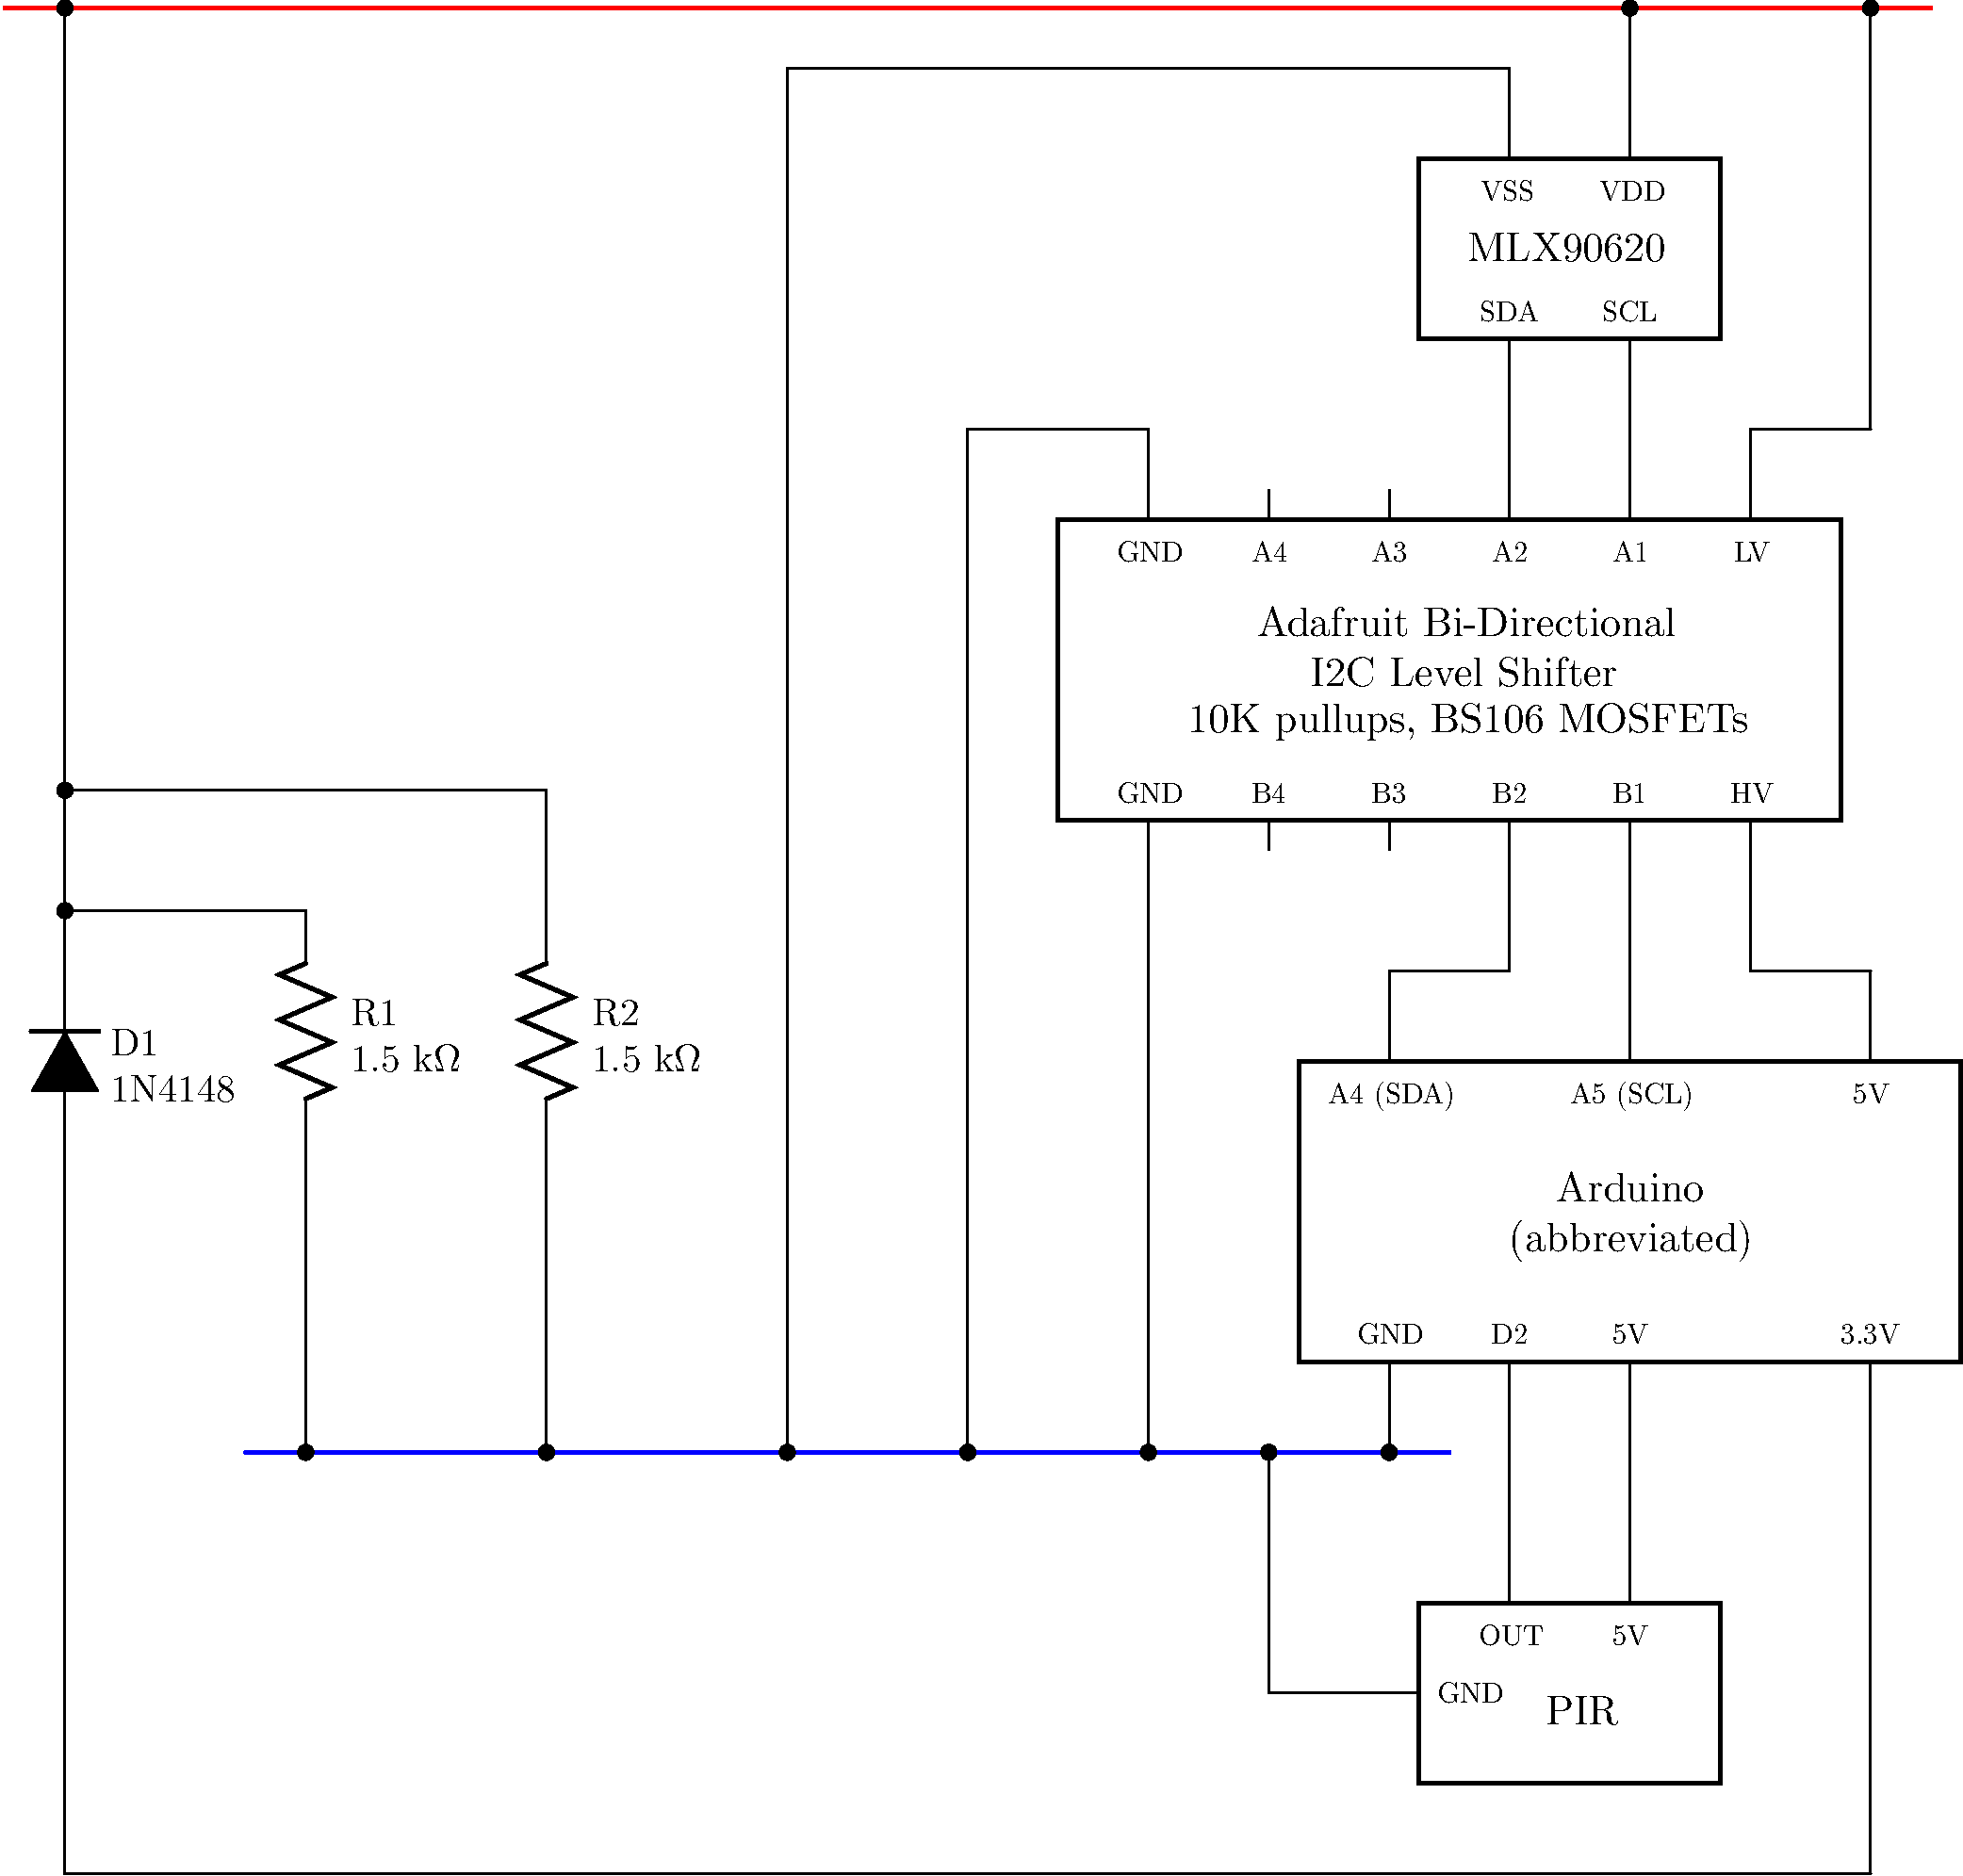
\includegraphics[width=\textwidth]{../diagrams/mlx-arduino2.pdf}
\caption{MLX90620, PIR and Arduino integration circuit}
\label{fig:circuits:node}
\end{figure}

Due to low cost and ease of use, the \ard platform was selected as the host for the Preprocessing Tier, and thus the low-level \iic interface for communication to the \mlx. Initially, this presented some challenges, as the \mlx recommends a power and communication voltage of 2.6V, while the \ard is only able to output 3.3V and 5V as power, and 5V as communication. Due to this, it was not possible to directly connect the \ard to the \mlx, and similarly due to the two-way nature of the \iic 2-wire communication protocol, it was also not possible to simply lower the \ard voltage using simple electrical techniques, as such techniques would interfere with two-way communication.

A solution was found in the form of a \iic level-shifter, the Adafruit ``4-channel I2C-safe Bi-directional Logic Level Converter'' \cite{AdafruitI2C}, which provided a cheap method to bi-directionally communicate between the two devices at their own preferred voltages. The layout of the circuit necessary to link the \ard and the \mlx using this converter can be seen in \Fref{fig:circuits:node}.

% TODO: Check PIR settings
Additionally, as used in the Thermosense paper, a \pir motion sensor \cite{AdafruitPIR} was also connected to the \ard. This sensor, operating at 5V natively, did not require any complex circuitry to interface with the \ard. It is connected to digital pin 2 on the \ard, where it provides a rising signal in the event that motion is detected, which can be configured to cause an interrupt on the \ard. In the configuration used in this project, the sensor's sensitivity was set to the highest value and the timeout for re-triggering was set to the lowest value (approximately 2.5 seconds). Additionally, the continuous re-triggering feature (whereby the sensor produces continuous rising and falling signals for the duration of motion) was disabled using the provided jumpers. 

% Talk about RPi and prototype board, and prototype iterations

For the Analysis Tier, the Raspberry Pi B+ was chosen, as it is a powerful computer capable of running Linux available for an extraordinarily low price. The \ard is connected to the Raspberry Pi over USB, which provides it both power and the capacity to transfer data. In turn, the Raspberry Pi is connected to a simple micro-USB rechargeable battery pack, which provides it with power, and subsequently the \ard and sensors.

\section{Software}

At each layer of the described three-tier software architecture (pictured in greater detail in \Fref{fig:pictures:protob-arch}), there must exist software which governs the operation of that tier's processing concerns. Software in this project was written in two different languages.

At the Sensing Tier, it was not necessary for any software to be developed, as any software necessary came pre-installed and ready for use on the aforementioned sensors.

At the Preprocessing Tier, the Arduino, the default C++ derivative language was used, as careful management of memory usage and algorithmic complexity is required in such a resource-constrained environment, thus limiting choice in the area.

Finally, at Analysis Tier, a computer running fully-fledged Linux, choice of language becomes a possibility. In this instance, Python was settled on as the language of choice, as it is a quite high-level language with excellent library support for the functions required of the Analysis Tier, including serial interface, the use of the Raspberry Pi's built in camera, and image analysis. The 2.x branch of Python was chosen over the 3.x branch, despite its age, due a greater maturity in support for several key graphical interface libraries.

\begin{figure}
\centering
\begin{tikzpicture}[node distance=1.7cm]
\node (interwebs) [cbox] {Network};
\node (wifi) [dashbox, right=of interwebs] {\small WiFi / Ethernet};
\node (rpi) [fcont, below=of wifi] {Raspberry Pi B+ \linebreak
  ``Analysis Tier'' \linebreak
  
  \tikz\node[fbox, minimum width=2.3cm, text width=2.3cm] {\small \ttfamily thinglib};
  \tikz\node[fbox, minimum width=2.3cm, text width=2.3cm] {\small \ttfamily features.py};
};
\node (cam) [box, right=of rpi] {Camera};
\node (usb) [dashbox, below=of rpi] {\small Serial over USB};
\node (ard) [fcont, below=of usb] {Arduino Uno R3 \linebreak
  ``Preprocessing Tier'' \linebreak
  
  \tikz\node[fbox, minimum width=3.8cm, text width=3.8cm] {\small \ttfamily mlx90620\_driver.ino};
};
\node (iic) [dashbox, left=of ard] {\small \iic};
\node (mlx) [box, below=of iic] {MLX90620};
\node (wire) [dashbox, right=of ard] {\small Interrupt};
\node (pir) [box, below=of wire] {PIR};
\node (sensetier) [dashbox, dotted, fit=(pir) (mlx)] {``Sensing Tier''};

\draw [line] (interwebs) -- (wifi);
\draw [line] (wifi) -- (rpi);
\draw [line] (rpi) -- (usb);
\draw [line] (usb) -- (ard);
\draw [line] (ard) -- (iic);
\draw [line] (iic) -- (mlx);
\draw [line] (ard) -- (wire);
\draw [line] (wire) -- (pir);
\draw [line] (rpi) -- (cam);
\end{tikzpicture}
\caption{Prototype system architecture}
\label{fig:pictures:protob-arch}
\end{figure}

\subsection{Pre-processing: \texttt{mlx90620\_driver.ino}}

On the Arduino, once large program was developed, termed \texttt{mlx90620\_driver.ino}. This program's purpose was to take simple commands over serial to configure the \mlx and to report back the current temperature values and \pir motion information at either a pre-set interval, or when requested.

To calculate the final temperature values that the \mlx offers, a complex initialization and computational process must be followed, which is specified in the sensor's datasheet \cite{MLXDatasheet}. This process involves initializing the sensor with values attained from a separate on-board \iic EEPROM, then retrieving a variety of normalization and adjustment values, along with the raw sensor data, to compute the final temperature result.

The basic algorithm to perform this normalization was based upon the provided datasheet \cite{MLXDatasheet}, as well as code by users ``maxbot'', ``IIBaboomba'', ``nseidle'' and others on the Arduino Forums \cite{ArduinoForum} and was modified to operate with the newer \ard ``Wire'' \iic libraries released since the authors' posts. In pursuit of the project's aims to create a more approachable thermal sensor, the code was also restructured and rewritten to be both more readable, and to introduce a set of features to make the management of the sensor data easier for the user, and for the information to be more human readable.

Additionally, support for the \pir's motion data was added to the code, with the \pir configured to perform interrupts on one of the Arduino's digital pinsnd the code structured to take note of this information and to report it to the user in the ``MOTION'' section of the next packet.

The first of the features introduced was the human-readable format for serial transmission. This allows the user to both easily write code that can parse the serial to acquire the serial data, as well as examine the serial data directly with ease. When the \ard first boots running the software, the output in \Fref{fig:code:initseq} is output. This specifies several things that are useful to the user; the attached sensor (``DRIVER''), the build of the software (``BUILD'') and the refresh rate of the sensor (``IRHZ''). Several different headers, such as ``ACTIVE'' and ``INIT'' specify the current millisecond time of the processor, thus indicating how long the execution of the initialization process took (33 milliseconds).

Once booted, the user is able to send several one-character commands to the sensor to configure operation, which are described in \Fref{tab:ardcommands}. Depending on the sensor configuration, IR data may be periodically output automatically, or otherwise manually triggered. This IR data is produced in the packet format described in \Fref{fig:code:initseq}. This is a simple, human readable format that includes the millisecond time of the processor at the start and end of the calculation, if the \pir has seen any motion for the duration of the calculation, and the 16x4 grid of calculated temperature values.

\begin{figure}
 \centering
\begin{minted}[frame=single,fontsize=\scriptsize]{text}
INIT 0
INFO START
DRIVER MLX90620
BUILD Feb  1 2015 00:00:00
IRHZ 1
INFO STOP
ACTIVE 33

START 34
MOVEMENT 0
1.0  1.0  1.0  1.0  1.0  1.0  1.0  1.0  1.0  1.0  1.0  1.0  1.0  1.0  1.0  1.0
1.0  1.0  1.0  1.0  1.0  1.0  1.0  1.0  1.0  1.0  1.0  1.0  1.0  1.0  1.0  1.0
1.0  1.0  1.0  1.0  1.0  1.0  1.0  1.0  1.0  1.0  1.0  1.0  1.0  1.0  1.0  1.0
1.0  1.0  1.0  1.0  1.0  1.0  1.0  1.0  1.0  1.0  1.0  1.0  1.0  1.0  1.0  1.0
STOP 97
\end{minted}
%\begin{tabular}{|l|l|}
%\hline
%\texttt{R} & Flush buffers and reset \ard \\ \hline
%\texttt{I} & Print INFO again \\ \hline
%\texttt{T} & Activate timers for periodic IR data output \\ \hline
%\texttt{O} & Deactivate timers for periodic IR data output \\ \hline
%\texttt{P} & Manually trigger capture and output of IR data \\ \hline
%\texttt{F\textit{x}} & Set sensor refresh frequency to \textit{x} and reboot \\ \hline
%\end{tabular}
\caption{Initialisation sequence and thermal packet}
\label{fig:code:initseq}
\end{figure}

\subsection{Analysis: \texttt{thinglib}}

On the analysis tier a set of Python libraries and accompanying utility scripts were developed to interface with the Arduino, parse and interpret its data, and to provide data logging and visualization capabilities. Most of this functionality was split into a reusable and versatile Python module called \texttt{thinglib}.

\texttt{thinglib} provides 4 main feature sets across 3 files; the \texttt{Manager} series of classes, the \texttt{Visualizer} class, the \texttt{Features} class and the \texttt{pxdisplay} module.

\subsubsection{\texttt{Manager} classes}
The Manager series of classes are the direct interface between the Arduino and the Python classes. They implement a multi-threaded serial data collection and parsing system which converts the raw serial output of the connected Arduino into a series of Python data structures that represent the collected temperature and motion data of each captured frame. Several different versions of the \texttt{Manager} class exist to perform slightly different functions. When initializing these classes the sample rate of the \mlx can be configured, and it will be sent through to the Arduino for updating.

\texttt{BaseManager} is responsible for the implementation of the core serial parsing functions. It also provides a threaded interface through which the \mlx's continuous stream of data can be subscribed to by other threads. The primary API, the \texttt{subscribe\_} series of functions, return a thread-safe queue structure, through which thermal packets can be received by various other threads when they become available.

\texttt{Manager}, the primary class, provides access the \mlx's data at configurable intervals. When initializing this class, you may specific 0.5, 1, 2, 4 or 8Hz, and the class will configure the Arduino to both set the \mlx to this sample rate, and to automatically write this data to the serial buffer whenever it is available. This serial interface is multi-threaded, as at higher serial baud rates if data was not polled continuously enough the internal serial buffer would fill and some data would be discarded. By ensuring this process cannot be blocked by other parts of the running program this problem is mostly eliminated. 

\texttt{OnDemandManager} operates in a similar way to \texttt{Manager}, however instead of using a non-blocking threaded approach, the user's scripts may request thermal/motion data from the class, and it will poll the Arduino for information and block until this information is parsed and returned.

Finally, \texttt{ManagerPlaybackEmulator} is a simple class which can take a previously created thermal recording from a file, and emulate the \texttt{Manager} class by providing access to thread-safe queues which return this data at the specified Hz rate. This class can be used as a means to playback thermal recordings with the same visualization functions.

\subsubsection{\texttt{pxdisplay} functions}

The \texttt{pxdisplay} module is a set of functions that utilize the \texttt{pygame} library to create a simple live-updating window containing a thermal map representation of the thermal data. One can generate any number of \texttt{pxdisplay} objects, which leverage the \texttt{multithreading} library and \texttt{multithreading.Queue} to allow thermal data to be sent to the display.

The class also provides a set of functions to set a ``hotest'' and ``coldest'' temperature and have RGB colors assigned from red to blue for each temperature that falls between those two extremes.

\subsubsection{\texttt{Visualizer} class}
The \texttt{Visualizer} class is the natural compliment to the \texttt{Manager} series of classes. The functions contained within can usually be provided with a Queue object (generated by a \texttt{Manager} class) and can perform a variety of visualization and storage functions.

From the recording side, the \texttt{Visualizer} class can ``record'' a thermal capture by saving the motion and thermal information to a simple \texttt{.tcap} file, which stores the sample rate, timings, thermal and motion data from a capture in a very straightforward format. The class can also read these files back into the data structures \texttt{Visualizer} uses internally to store data. If \texttt{Visualizer} is running on a Raspberry Pi, it can also leverage the \texttt{picamera} library an the \texttt{OnDemandManager} class to synchronously capture both visual and thermal data for ground truth purposes.

From the visualization side, \texttt{Visualizer} can leverage the \texttt{pxdisplay} module to create thermal maps that can update in real-time based on the thermal data provided by a \texttt{Manager} class. The class can also generate both images and movie files from thermal recordings using the PIL and ffmpeg libraries respectively.

\subsubsection{\texttt{Features} class}

In Thermosense \cite{beltran2013thermosense}, an algorithm was demonstrated that allowed the separation of ``background'' information from ``active'' pixels, and from that information, the extraction of the features necessary for a classifier to correctly determine the number of people in an $8\times8$ thermal image. This algorithm involved calculating the average and standard deviations of each pixel while it is guaranteed that the image would be empty, and then when motion is detected, considering any pixel ``active'' that reaches a value more than 3 standard deviations above the pixel when there was no motion.

From these ``active'' pixels, it was established that a set of three feature vectors were all that were required to correctly classify the number of people in the thermal image. These feature vectors were;
\begin{enumerate}
\item \textbf{Number of active pixels}: The total number of pixels that are considered ``active'' in a given frame
\item \textbf{Number of connected components}: If each active pixel is represented as an node in an undirected graph where adjacent active pixels are connected, how many connected components does this graph have?
\item \textbf{Size of largest connected component}: The number of active pixels contained within the largest connected component
\end{enumerate}

In accordance with the pseudo-code outlined in the Thermosense paper, the algorithm described in \Fref{lst:exps:featcode} was created to extract these figures. The portion of this code dealing with scaling the thermal background for rooms without motion was not implemented, as in all experiments tested, there exists a significant interval of time during which the no motion is guarenteed and the thermal background can be generated. The \texttt{networkx} library was used to generate the connected components information.

\begin{listing}
\centering
\begin{minted}[fontsize=\footnotesize,frame=single,breaklines=true]{python}
import networkx, itertools

nomotion_wgt = 0.01
n_rows = 4
n_cols = 16
background = first_frame
means = first_frame
stds = [ [0]*16 ]*4
stds_post = [ [None]*16 ]*4

def create_features(new_frame, is_motion):
  active = []
  g = networkx.Graph()

  for i, j in itertools.product( range(n_rows), range(n_cols) ):
    prev = background[i][j]
    cur = new_frame[i][j]
    cur_mean = means[i][j]
    cur_std = stds[i][j]

    if not is_motion:
      background[i][j] = nomotion_wgt * cur + (1 - nomotion_wgt) * prev
      means[i][j]      = cur_mean + (cur - cur_mean) / n
      stds[i][j]       = cur_std + (cur - cur_mean) * (cur - means[i][j])
      stds_post[i][j]  = math.sqrt(stds[i][j] / (n-1))

    if (cur - background[i][j]) > (3 * stds_post[i][j]):
      active.append((i,j))
      g.add_node((i,j))

      # Add edges for nodes that have already been computed as active
      for ix, jx in [(-1, -1), (-1, 0), (-1, 1), (0, -1)]:
        if (i+ix, j+jx) in active:
          g.add_edge((i,j), (i+ix,j+jx))

  comps = list(networkx.connected_components(g))
  num_active = len(active)
  num_connected = len(comps)
  size_connected = max(len(c) for c in comps) if len(comps) > 0 else None

  return (num_active, num_connected, size_connected)
\end{minted}
\caption{Core feature extraction code}
\label{lst:exps:featcode}
\end{listing}

\clearpage

% TODO Talk about ground truth generation script

\section{Sensor Properties}

In order to best utilize the \mlx, we must first understand the properties it exhibits, and their potential affects on our ability to perform person related measurements. These properties can be broadly separated into three different categories; bias, noise and sensitivity. A broad range of data was collected with the sensor in a horizontal orientation using various sources of heat and cold to determine these properties. This experimental setup is described in \Fref{fig:exps:2setup}.

\begin{figure}
\centering
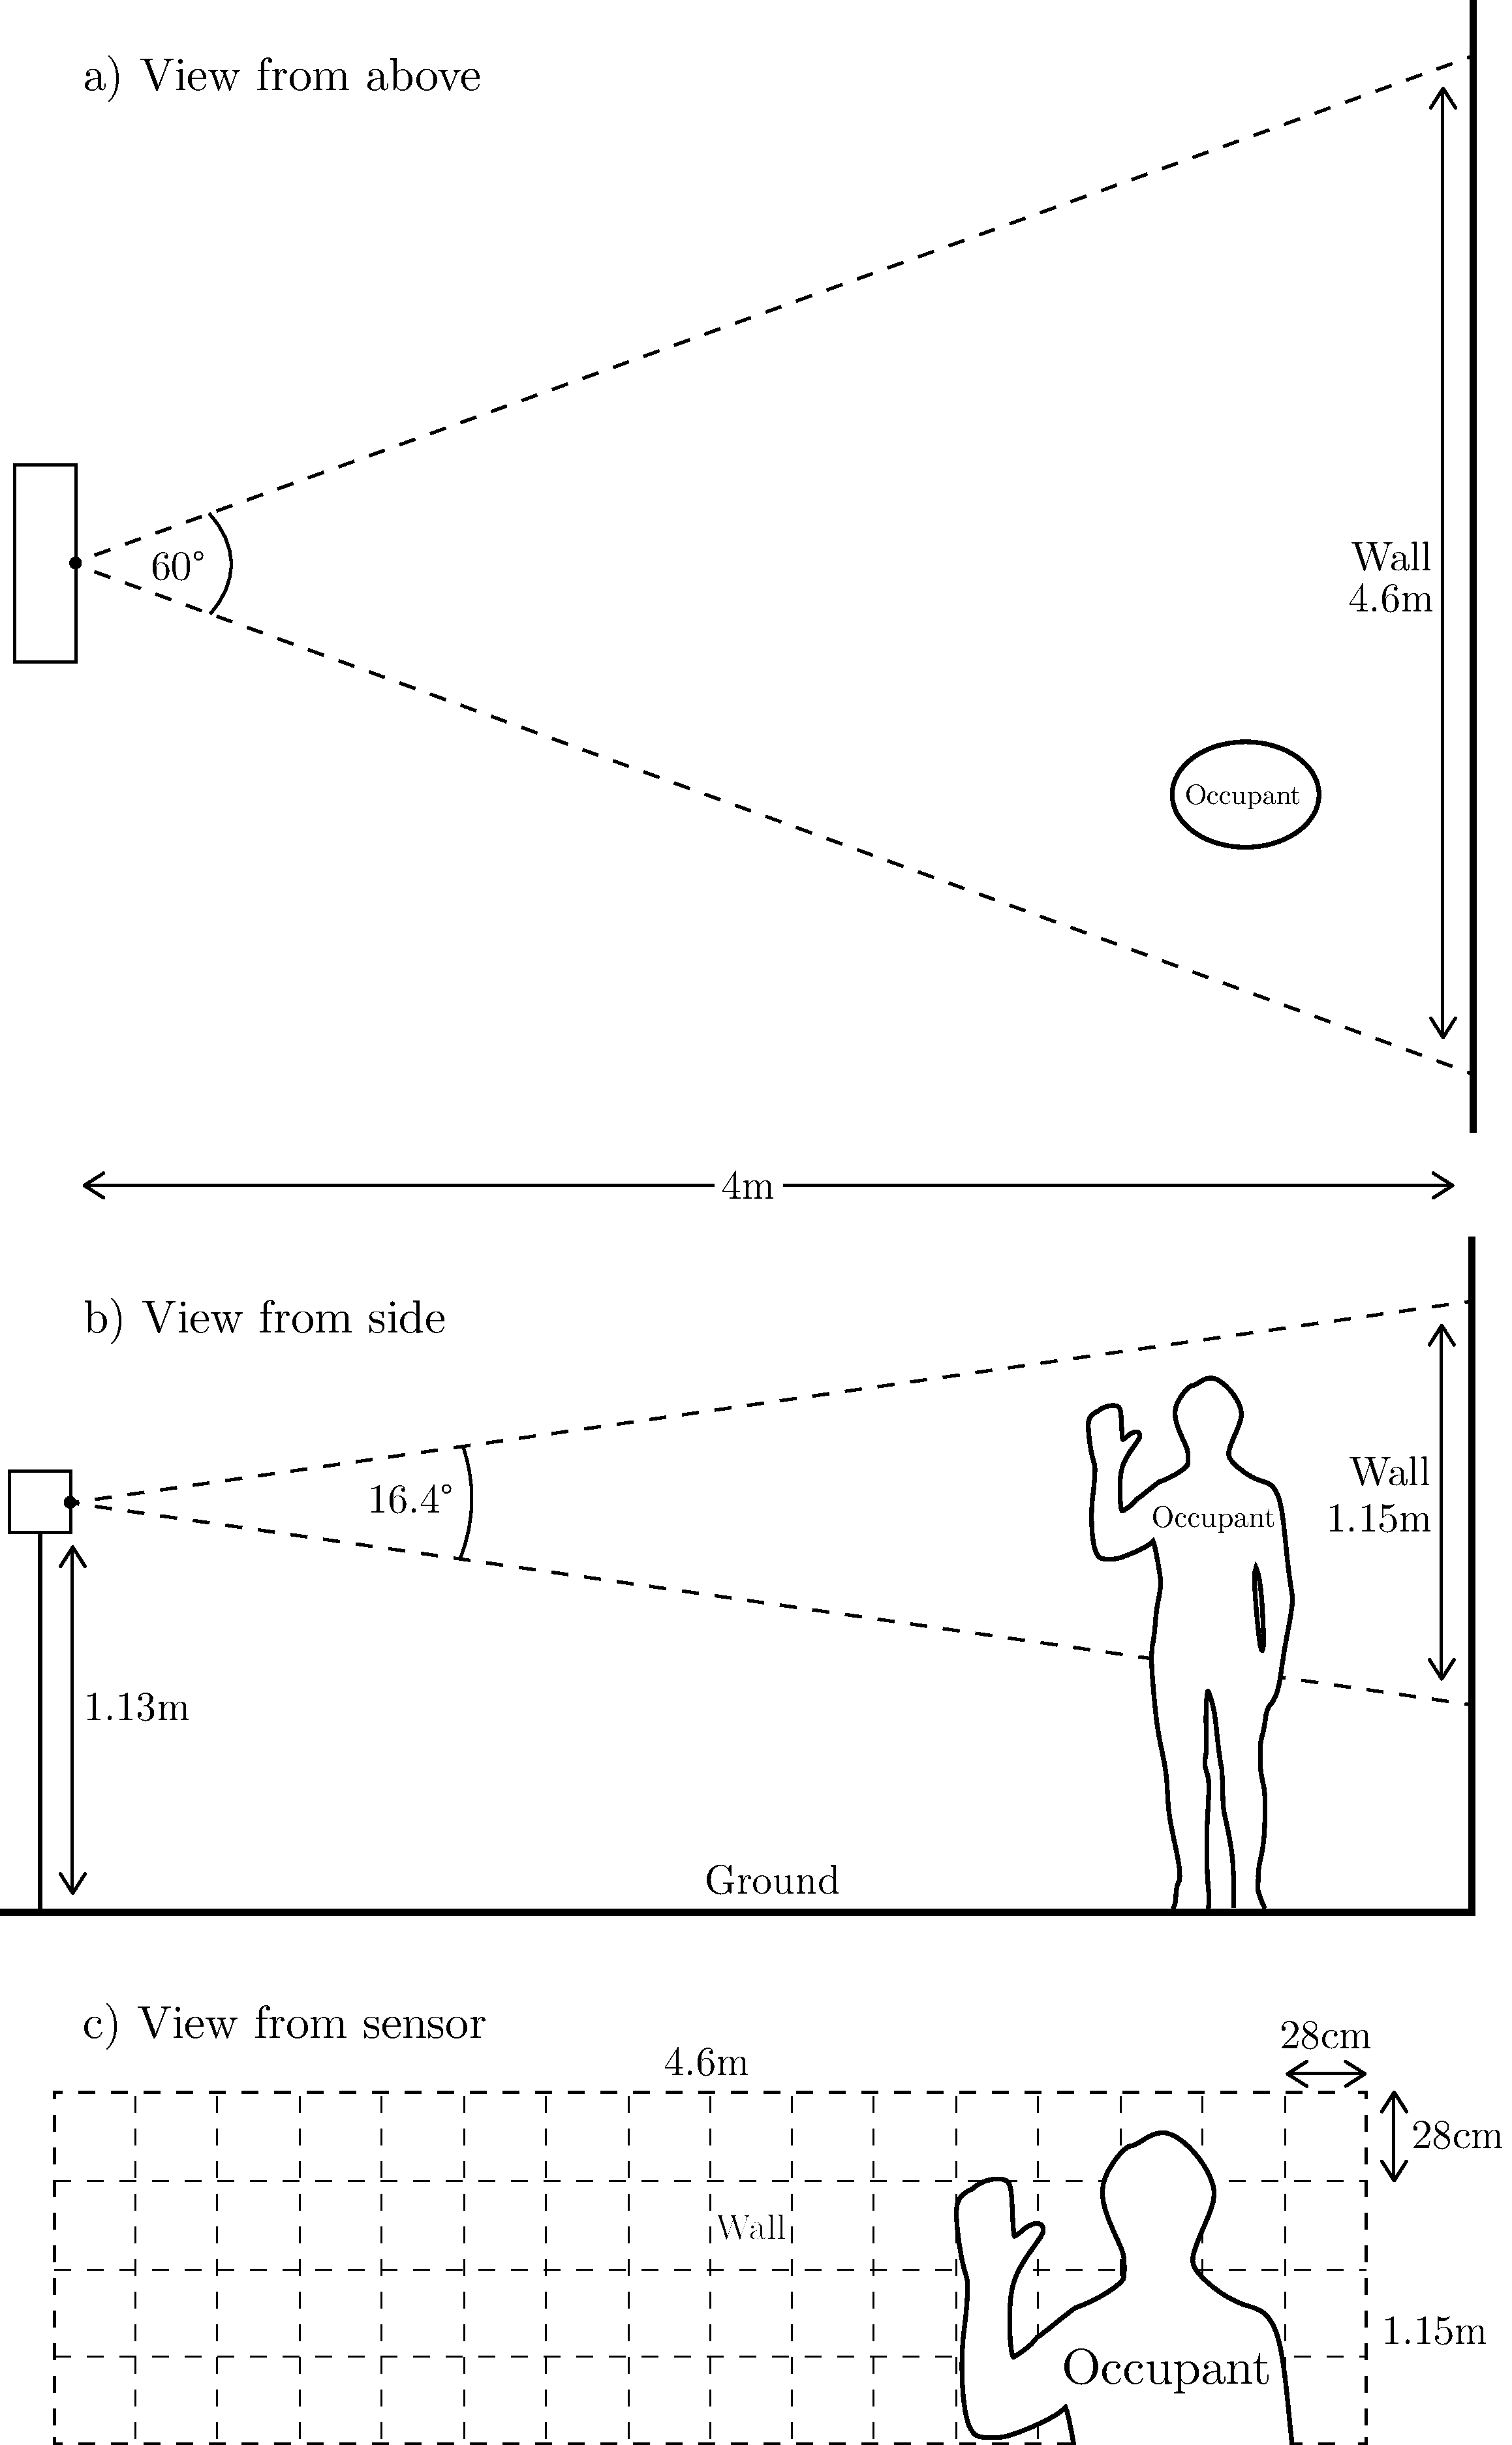
\includegraphics[height=0.9\textheight]{../diagrams/second-exp-setup2.pdf}
\caption{Experiment setup to determine sensor properties}
\label{fig:exps:2setup}
\end{figure}


\subsection{Bias}
When receiving no infrared radiation, the sensor should indicate a near-zero temperature. If in such conditions it does not, that indicates that the sensor has some level of bias in its measurement values. We attempted to investigate this bias by performing thermal captures of the night sky. While this does not completely remove the infrared radiation, it does remove a significant proportion of it.

In \Fref{tab:meanstd} the thermal sensor was exposed to the night sky at a capture rate of 1Hz for 4 minutes, with the sensing results combined to create a set of means and standard deviations to indicate the pixels at ``rest''. The average temperature detected was $11.78\dc$, with the standard deviation remaining less than $0.51\dc$ over the entire exposure period. The resultant thermal map shows that pixels centered around the four ``primary'' pixels in the center maintain a similar temperature around $9\dc$, with temperatures beginning to deviate as they became further from the center.

The most likely cause of this bias is related to the physical structure of the sensor. The \mlx is a rectangular sensor which has been placed inside a circular tube. Due to this physical arrangement, the sides of this rectangular sensor will be significantly closer to these edges than the center. If these sides are at an ambient temperature higher than the measurement data (as they were in this case) thermal radiation from the sensor package itself could provide significant enough to cause the edges to appear warmer than the observed area of the sky. Such issues with temperature could be controlled for using a device that cools the sensor package to below that of the ambient temperature being measured, however, this is not a concern in this project, as the method of calculating a thermal background will compensate for any such bias as long as it remains constant.

\begin{landscape}
\begin{table}
\centering
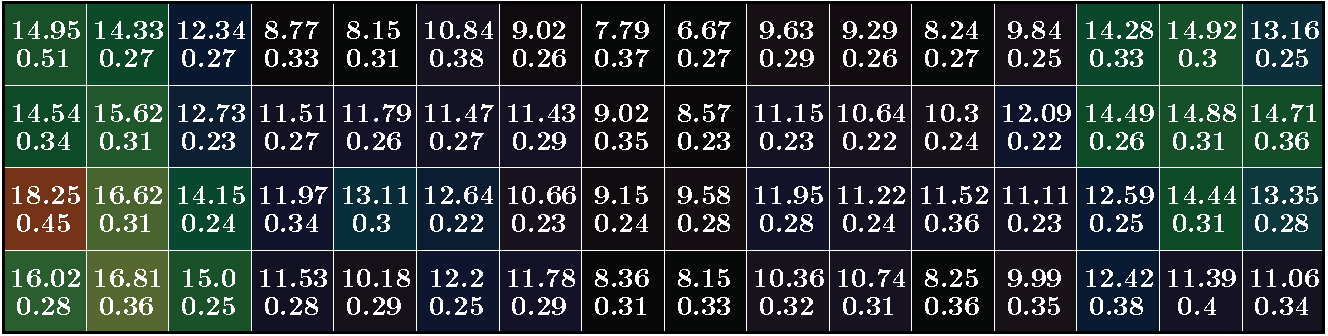
\includegraphics{../diagrams/sensor-bias-thermal-map.pdf}
\caption{Mean and standard deviations for each pixel at rest}
\label{tab:meanstd}
\end{table}
\end{landscape}


\subsection{Noise}

One of the features of the \mlx is the ability to sample the thermal data and a variety of sample rates between 0.5Hz and 512Hz. However, it was noted in early experimentation that a higher sample rate resulted in an increase in the noise contained within the resultant images. As our experiments focus on separating objects of interest from a thermal background, it is important to determine the maximum level of noise tolerable before our algorithms are unable to separate the background from the objects of interest.

\Fref{fig:noise} plots one of the central pixels of the sensor in a scenario where it is merely viewing a background (shown in green), and when it is viewing a person (shown in red), at the 5 different sample rates achievable with the current hardware. We can see in these plots that the data becomes significantly more noisy as the sample rate increases, and we can also determine that the sensor uses a form of data smoothing at lower sample rates, as the variance in data increases with sample rate.

If the sample rate were to increase, it is likely that the ability for the sensing system to disambiguate between objects of interest and the background would diminish. However, in the current project, even the slowest sampling rate of 0.5Hz is sufficient, as occupancy estimations at a sub-second level present little additional value and would require significant reforms in the efficiency of the software used.

% TODO: Signal to noise ratio calculations

\begin{figure}
  \centering
  \begin{tikzpicture}[gnuplot]
%% generated with GNUPLOT 4.6p6 (Lua 5.2; terminal rev. 99, script rev. 100)
%% 26/03/2015 10:45:05 AM
\tikzset{every node/.append style={font={\fontsize{9pt}{10.8pt}\selectfont}}}
\gpmonochromelines
\path (0.000,0.000) rectangle (12.700,19.050);
\gpcolor{rgb color={0.502,0.502,0.502}}
\gpsetlinetype{gp lt axes}
\gpsetlinewidth{1.00}
\draw[gp path] (0.498,15.794)--(12.201,15.794);
\gpcolor{color=gp lt color border}
\node[gp node right,font={\fontsize{8pt}{9.6pt}\selectfont}] at (0.332,15.794) {};
\gpcolor{rgb color={0.502,0.502,0.502}}
\draw[gp path] (0.498,16.445)--(12.201,16.445);
\gpcolor{color=gp lt color border}
\node[gp node right,font={\fontsize{8pt}{9.6pt}\selectfont}] at (0.332,16.445) {};
\gpcolor{rgb color={0.502,0.502,0.502}}
\draw[gp path] (0.498,17.096)--(12.201,17.096);
\gpcolor{color=gp lt color border}
\node[gp node right,font={\fontsize{8pt}{9.6pt}\selectfont}] at (0.332,17.096) {};
\gpcolor{rgb color={0.502,0.502,0.502}}
\draw[gp path] (0.498,17.747)--(12.201,17.747);
\gpcolor{color=gp lt color border}
\node[gp node right,font={\fontsize{8pt}{9.6pt}\selectfont}] at (0.332,17.747) {};
\gpcolor{rgb color={0.502,0.502,0.502}}
\draw[gp path] (0.498,18.398)--(12.201,18.398);
\gpcolor{color=gp lt color border}
\node[gp node right,font={\fontsize{8pt}{9.6pt}\selectfont}] at (0.332,18.398) {};
\gpcolor{rgb color={0.502,0.502,0.502}}
\draw[gp path] (0.498,19.049)--(12.201,19.049);
\gpcolor{color=gp lt color border}
\node[gp node right,font={\fontsize{8pt}{9.6pt}\selectfont}] at (0.332,19.049) {};
\gpcolor{rgb color={0.502,0.502,0.502}}
\draw[gp path] (1.229,15.794)--(1.229,19.049);
\gpcolor{color=gp lt color border}
\node[gp node center,font={\fontsize{8pt}{9.6pt}\selectfont}] at (1.229,15.517) { 5};
\gpcolor{rgb color={0.502,0.502,0.502}}
\draw[gp path] (2.449,15.794)--(2.449,19.049);
\gpcolor{color=gp lt color border}
\node[gp node center,font={\fontsize{8pt}{9.6pt}\selectfont}] at (2.449,15.517) { 10};
\gpcolor{rgb color={0.502,0.502,0.502}}
\draw[gp path] (3.668,15.794)--(3.668,19.049);
\gpcolor{color=gp lt color border}
\node[gp node center,font={\fontsize{8pt}{9.6pt}\selectfont}] at (3.668,15.517) { 15};
\gpcolor{rgb color={0.502,0.502,0.502}}
\draw[gp path] (4.887,15.794)--(4.887,19.049);
\gpcolor{color=gp lt color border}
\node[gp node center,font={\fontsize{8pt}{9.6pt}\selectfont}] at (4.887,15.517) { 20};
\gpcolor{rgb color={0.502,0.502,0.502}}
\draw[gp path] (6.106,15.794)--(6.106,19.049);
\gpcolor{color=gp lt color border}
\node[gp node center,font={\fontsize{8pt}{9.6pt}\selectfont}] at (6.106,15.517) { 25};
\gpcolor{rgb color={0.502,0.502,0.502}}
\draw[gp path] (7.325,15.794)--(7.325,19.049);
\gpcolor{color=gp lt color border}
\node[gp node center,font={\fontsize{8pt}{9.6pt}\selectfont}] at (7.325,15.517) { 30};
\gpcolor{rgb color={0.502,0.502,0.502}}
\draw[gp path] (8.544,15.794)--(8.544,19.049);
\gpcolor{color=gp lt color border}
\node[gp node center,font={\fontsize{8pt}{9.6pt}\selectfont}] at (8.544,15.517) { 35};
\gpcolor{rgb color={0.502,0.502,0.502}}
\draw[gp path] (9.763,15.794)--(9.763,19.049);
\gpcolor{color=gp lt color border}
\node[gp node center,font={\fontsize{8pt}{9.6pt}\selectfont}] at (9.763,15.517) { 40};
\gpcolor{rgb color={0.502,0.502,0.502}}
\draw[gp path] (10.982,15.794)--(10.982,19.049);
\gpcolor{color=gp lt color border}
\node[gp node center,font={\fontsize{8pt}{9.6pt}\selectfont}] at (10.982,15.517) { 45};
\gpcolor{rgb color={0.502,0.502,0.502}}
\draw[gp path] (12.201,15.794)--(12.201,19.049);
\gpcolor{color=gp lt color border}
\node[gp node center,font={\fontsize{8pt}{9.6pt}\selectfont}] at (12.201,15.517) { 50};
\node[gp node left,font={\fontsize{8pt}{9.6pt}\selectfont}] at (12.367,15.794) { 26};
\node[gp node left,font={\fontsize{8pt}{9.6pt}\selectfont}] at (12.367,16.445) { 28};
\node[gp node left,font={\fontsize{8pt}{9.6pt}\selectfont}] at (12.367,17.096) { 30};
\node[gp node left,font={\fontsize{8pt}{9.6pt}\selectfont}] at (12.367,17.747) { 32};
\node[gp node left,font={\fontsize{8pt}{9.6pt}\selectfont}] at (12.367,18.398) { 34};
\node[gp node left,font={\fontsize{8pt}{9.6pt}\selectfont}] at (12.367,19.049) { 36};
\gpsetlinetype{gp lt border}
\draw[gp path] (0.498,19.049)--(0.498,15.794)--(12.201,15.794)--(12.201,19.049)--cycle;
\node[gp node center,rotate=-270] at (0.027,17.421) {0.5 Hz};
\gpcolor{rgb color={0.400,0.651,0.118}}
\gpsetlinetype{gp lt plot 0}
\draw[gp path] (0.498,16.305)--(0.986,16.334)--(1.473,16.305)--(1.961,16.364)--(2.449,16.396)%
  --(2.936,16.409)--(3.424,16.334)--(3.911,16.347)--(4.399,16.305)--(4.887,16.318)--(5.374,16.380)%
  --(5.862,16.334)--(6.350,16.289)--(6.837,16.318)--(7.325,16.334)--(7.812,16.305)--(8.300,16.364)%
  --(8.788,16.364)--(9.275,16.334)--(9.763,16.347)--(10.251,16.347)--(10.738,16.334)--(11.226,16.334)%
  --(11.713,16.334)--(12.201,16.334);
\gpcolor{rgb color={0.906,0.161,0.541}}
\draw[gp path] (0.498,18.551)--(0.986,18.567)--(1.473,18.538)--(1.961,18.538)--(2.449,18.652)%
  --(2.936,18.652)--(3.424,18.665)--(3.911,18.551)--(4.399,18.567)--(4.887,18.665)--(5.374,18.551)%
  --(5.862,18.538)--(6.350,18.551)--(6.837,18.538)--(7.325,18.509)--(7.812,18.567)--(8.300,18.538)%
  --(8.788,18.551)--(9.275,18.652)--(9.763,18.597)--(10.251,18.639)--(10.738,18.681)--(11.226,18.681)%
  --(11.713,18.681)--(12.201,18.681);
\gpcolor{color=gp lt color border}
\gpsetlinetype{gp lt border}
\draw[gp path] (0.498,19.049)--(0.498,15.794)--(12.201,15.794)--(12.201,19.049)--cycle;
%% coordinates of the plot area
\gpdefrectangularnode{gp plot 1}{\pgfpoint{0.498cm}{15.794cm}}{\pgfpoint{12.201cm}{19.049cm}}
\gpcolor{rgb color={0.502,0.502,0.502}}
\gpsetlinetype{gp lt axes}
\draw[gp path] (0.498,11.984)--(12.201,11.984);
\gpcolor{color=gp lt color border}
\node[gp node right,font={\fontsize{8pt}{9.6pt}\selectfont}] at (0.332,11.984) {26};
\gpcolor{rgb color={0.502,0.502,0.502}}
\draw[gp path] (0.498,12.635)--(12.201,12.635);
\gpcolor{color=gp lt color border}
\node[gp node right,font={\fontsize{8pt}{9.6pt}\selectfont}] at (0.332,12.635) {28};
\gpcolor{rgb color={0.502,0.502,0.502}}
\draw[gp path] (0.498,13.286)--(12.201,13.286);
\gpcolor{color=gp lt color border}
\node[gp node right,font={\fontsize{8pt}{9.6pt}\selectfont}] at (0.332,13.286) {30};
\gpcolor{rgb color={0.502,0.502,0.502}}
\draw[gp path] (0.498,13.937)--(12.201,13.937);
\gpcolor{color=gp lt color border}
\node[gp node right,font={\fontsize{8pt}{9.6pt}\selectfont}] at (0.332,13.937) {32};
\gpcolor{rgb color={0.502,0.502,0.502}}
\draw[gp path] (0.498,14.588)--(12.201,14.588);
\gpcolor{color=gp lt color border}
\node[gp node right,font={\fontsize{8pt}{9.6pt}\selectfont}] at (0.332,14.588) {34};
\gpcolor{rgb color={0.502,0.502,0.502}}
\draw[gp path] (0.498,15.239)--(12.201,15.239);
\gpcolor{color=gp lt color border}
\node[gp node right,font={\fontsize{8pt}{9.6pt}\selectfont}] at (0.332,15.239) {36};
\gpcolor{rgb color={0.502,0.502,0.502}}
\draw[gp path] (1.229,11.984)--(1.229,15.239);
\gpcolor{color=gp lt color border}
\node[gp node center,font={\fontsize{8pt}{9.6pt}\selectfont}] at (1.229,11.707) { 5};
\gpcolor{rgb color={0.502,0.502,0.502}}
\draw[gp path] (2.449,11.984)--(2.449,15.239);
\gpcolor{color=gp lt color border}
\node[gp node center,font={\fontsize{8pt}{9.6pt}\selectfont}] at (2.449,11.707) { 10};
\gpcolor{rgb color={0.502,0.502,0.502}}
\draw[gp path] (3.668,11.984)--(3.668,15.239);
\gpcolor{color=gp lt color border}
\node[gp node center,font={\fontsize{8pt}{9.6pt}\selectfont}] at (3.668,11.707) { 15};
\gpcolor{rgb color={0.502,0.502,0.502}}
\draw[gp path] (4.887,11.984)--(4.887,15.239);
\gpcolor{color=gp lt color border}
\node[gp node center,font={\fontsize{8pt}{9.6pt}\selectfont}] at (4.887,11.707) { 20};
\gpcolor{rgb color={0.502,0.502,0.502}}
\draw[gp path] (6.106,11.984)--(6.106,15.239);
\gpcolor{color=gp lt color border}
\node[gp node center,font={\fontsize{8pt}{9.6pt}\selectfont}] at (6.106,11.707) { 25};
\gpcolor{rgb color={0.502,0.502,0.502}}
\draw[gp path] (7.325,11.984)--(7.325,15.239);
\gpcolor{color=gp lt color border}
\node[gp node center,font={\fontsize{8pt}{9.6pt}\selectfont}] at (7.325,11.707) { 30};
\gpcolor{rgb color={0.502,0.502,0.502}}
\draw[gp path] (8.544,11.984)--(8.544,15.239);
\gpcolor{color=gp lt color border}
\node[gp node center,font={\fontsize{8pt}{9.6pt}\selectfont}] at (8.544,11.707) { 35};
\gpcolor{rgb color={0.502,0.502,0.502}}
\draw[gp path] (9.763,11.984)--(9.763,15.239);
\gpcolor{color=gp lt color border}
\node[gp node center,font={\fontsize{8pt}{9.6pt}\selectfont}] at (9.763,11.707) { 40};
\gpcolor{rgb color={0.502,0.502,0.502}}
\draw[gp path] (10.982,11.984)--(10.982,15.239);
\gpcolor{color=gp lt color border}
\node[gp node center,font={\fontsize{8pt}{9.6pt}\selectfont}] at (10.982,11.707) { 45};
\gpcolor{rgb color={0.502,0.502,0.502}}
\draw[gp path] (12.201,11.984)--(12.201,15.239);
\gpcolor{color=gp lt color border}
\node[gp node center,font={\fontsize{8pt}{9.6pt}\selectfont}] at (12.201,11.707) { 50};
\gpsetlinetype{gp lt border}
\draw[gp path] (0.498,15.239)--(0.498,11.984)--(12.201,11.984)--(12.201,15.239)--cycle;
\node[gp node center,rotate=-270] at (12.476,13.611) {1 Hz};
\gpcolor{rgb color={0.400,0.651,0.118}}
\gpsetlinetype{gp lt plot 0}
\draw[gp path] (0.498,12.599)--(0.742,12.586)--(0.986,12.554)--(1.229,12.570)--(1.473,12.537)%
  --(1.717,12.508)--(1.961,12.554)--(2.205,12.508)--(2.449,12.479)--(2.692,12.524)--(2.936,12.615)%
  --(3.180,12.554)--(3.424,12.417)--(3.668,12.554)--(3.911,12.508)--(4.155,12.524)--(4.399,12.479)%
  --(4.643,12.508)--(4.887,12.599)--(5.130,12.508)--(5.374,12.615)--(5.618,12.495)--(5.862,12.449)%
  --(6.106,12.537)--(6.350,12.554)--(6.593,12.508)--(6.837,12.599)--(7.081,12.479)--(7.325,12.632)%
  --(7.569,12.479)--(7.812,12.495)--(8.056,12.508)--(8.300,12.508)--(8.544,12.508)--(8.788,12.554)%
  --(9.031,12.479)--(9.275,12.554)--(9.519,12.524)--(9.763,12.537)--(10.007,12.677)--(10.251,12.554)%
  --(10.494,12.537)--(10.738,12.615)--(10.982,12.554)--(11.226,12.462)--(11.470,12.479)--(11.713,12.508)%
  --(11.957,12.508)--(12.201,12.524);
\gpcolor{rgb color={0.906,0.161,0.541}}
\draw[gp path] (0.498,14.757)--(0.742,14.699)--(0.986,14.757)--(1.229,14.686)--(1.473,14.741)%
  --(1.717,14.686)--(1.961,14.741)--(2.205,14.686)--(2.449,14.871)--(2.692,14.728)--(2.936,14.770)%
  --(3.180,14.699)--(3.424,14.741)--(3.668,14.728)--(3.911,14.800)--(4.155,14.757)--(4.399,14.673)%
  --(4.643,14.741)--(4.887,14.673)--(5.130,14.757)--(5.374,14.715)--(5.618,14.770)--(5.862,14.715)%
  --(6.106,14.855)--(6.350,14.741)--(6.593,14.741)--(6.837,14.643)--(7.081,14.800)--(7.325,14.842)%
  --(7.569,14.686)--(7.812,14.699)--(8.056,14.673)--(8.300,14.757)--(8.544,14.686)--(8.788,14.741)%
  --(9.031,14.842)--(9.275,14.855)--(9.519,14.715)--(9.763,14.741)--(10.007,14.627)--(10.251,14.673)%
  --(10.494,14.741)--(10.738,14.673)--(10.982,14.757)--(11.226,14.673)--(11.470,14.627)--(11.713,14.559)%
  --(11.957,14.699)--(12.201,14.741);
\gpcolor{color=gp lt color border}
\gpsetlinetype{gp lt border}
\draw[gp path] (0.498,15.239)--(0.498,11.984)--(12.201,11.984)--(12.201,15.239)--cycle;
%% coordinates of the plot area
\gpdefrectangularnode{gp plot 2}{\pgfpoint{0.498cm}{11.984cm}}{\pgfpoint{12.201cm}{15.239cm}}
\gpcolor{rgb color={0.502,0.502,0.502}}
\gpsetlinetype{gp lt axes}
\draw[gp path] (0.498,8.174)--(12.201,8.174);
\gpcolor{color=gp lt color border}
\node[gp node right,font={\fontsize{8pt}{9.6pt}\selectfont}] at (0.332,8.174) {};
\gpcolor{rgb color={0.502,0.502,0.502}}
\draw[gp path] (0.498,8.825)--(12.201,8.825);
\gpcolor{color=gp lt color border}
\node[gp node right,font={\fontsize{8pt}{9.6pt}\selectfont}] at (0.332,8.825) {};
\gpcolor{rgb color={0.502,0.502,0.502}}
\draw[gp path] (0.498,9.476)--(12.201,9.476);
\gpcolor{color=gp lt color border}
\node[gp node right,font={\fontsize{8pt}{9.6pt}\selectfont}] at (0.332,9.476) {};
\gpcolor{rgb color={0.502,0.502,0.502}}
\draw[gp path] (0.498,10.127)--(12.201,10.127);
\gpcolor{color=gp lt color border}
\node[gp node right,font={\fontsize{8pt}{9.6pt}\selectfont}] at (0.332,10.127) {};
\gpcolor{rgb color={0.502,0.502,0.502}}
\draw[gp path] (0.498,10.778)--(12.201,10.778);
\gpcolor{color=gp lt color border}
\node[gp node right,font={\fontsize{8pt}{9.6pt}\selectfont}] at (0.332,10.778) {};
\gpcolor{rgb color={0.502,0.502,0.502}}
\draw[gp path] (0.498,11.429)--(12.201,11.429);
\gpcolor{color=gp lt color border}
\node[gp node right,font={\fontsize{8pt}{9.6pt}\selectfont}] at (0.332,11.429) {};
\gpcolor{rgb color={0.502,0.502,0.502}}
\draw[gp path] (1.229,8.174)--(1.229,11.429);
\gpcolor{color=gp lt color border}
\node[gp node center,font={\fontsize{8pt}{9.6pt}\selectfont}] at (1.229,7.897) { 5};
\gpcolor{rgb color={0.502,0.502,0.502}}
\draw[gp path] (2.449,8.174)--(2.449,11.429);
\gpcolor{color=gp lt color border}
\node[gp node center,font={\fontsize{8pt}{9.6pt}\selectfont}] at (2.449,7.897) { 10};
\gpcolor{rgb color={0.502,0.502,0.502}}
\draw[gp path] (3.668,8.174)--(3.668,11.429);
\gpcolor{color=gp lt color border}
\node[gp node center,font={\fontsize{8pt}{9.6pt}\selectfont}] at (3.668,7.897) { 15};
\gpcolor{rgb color={0.502,0.502,0.502}}
\draw[gp path] (4.887,8.174)--(4.887,11.429);
\gpcolor{color=gp lt color border}
\node[gp node center,font={\fontsize{8pt}{9.6pt}\selectfont}] at (4.887,7.897) { 20};
\gpcolor{rgb color={0.502,0.502,0.502}}
\draw[gp path] (6.106,8.174)--(6.106,11.429);
\gpcolor{color=gp lt color border}
\node[gp node center,font={\fontsize{8pt}{9.6pt}\selectfont}] at (6.106,7.897) { 25};
\gpcolor{rgb color={0.502,0.502,0.502}}
\draw[gp path] (7.325,8.174)--(7.325,11.429);
\gpcolor{color=gp lt color border}
\node[gp node center,font={\fontsize{8pt}{9.6pt}\selectfont}] at (7.325,7.897) { 30};
\gpcolor{rgb color={0.502,0.502,0.502}}
\draw[gp path] (8.544,8.174)--(8.544,11.429);
\gpcolor{color=gp lt color border}
\node[gp node center,font={\fontsize{8pt}{9.6pt}\selectfont}] at (8.544,7.897) { 35};
\gpcolor{rgb color={0.502,0.502,0.502}}
\draw[gp path] (9.763,8.174)--(9.763,11.429);
\gpcolor{color=gp lt color border}
\node[gp node center,font={\fontsize{8pt}{9.6pt}\selectfont}] at (9.763,7.897) { 40};
\gpcolor{rgb color={0.502,0.502,0.502}}
\draw[gp path] (10.982,8.174)--(10.982,11.429);
\gpcolor{color=gp lt color border}
\node[gp node center,font={\fontsize{8pt}{9.6pt}\selectfont}] at (10.982,7.897) { 45};
\gpcolor{rgb color={0.502,0.502,0.502}}
\draw[gp path] (12.201,8.174)--(12.201,11.429);
\gpcolor{color=gp lt color border}
\node[gp node center,font={\fontsize{8pt}{9.6pt}\selectfont}] at (12.201,7.897) { 50};
\node[gp node left,font={\fontsize{8pt}{9.6pt}\selectfont}] at (12.367,8.174) { 26};
\node[gp node left,font={\fontsize{8pt}{9.6pt}\selectfont}] at (12.367,8.825) { 28};
\node[gp node left,font={\fontsize{8pt}{9.6pt}\selectfont}] at (12.367,9.476) { 30};
\node[gp node left,font={\fontsize{8pt}{9.6pt}\selectfont}] at (12.367,10.127) { 32};
\node[gp node left,font={\fontsize{8pt}{9.6pt}\selectfont}] at (12.367,10.778) { 34};
\node[gp node left,font={\fontsize{8pt}{9.6pt}\selectfont}] at (12.367,11.429) { 36};
\gpsetlinetype{gp lt border}
\draw[gp path] (0.498,11.429)--(0.498,8.174)--(12.201,8.174)--(12.201,11.429)--cycle;
\node[gp node center,rotate=-270] at (0.027,9.801) {2 Hz};
\gpcolor{rgb color={0.400,0.651,0.118}}
\gpsetlinetype{gp lt plot 0}
\draw[gp path] (0.498,8.805)--(0.620,8.685)--(0.742,8.805)--(0.864,8.623)--(0.986,8.789)%
  --(1.108,8.789)--(1.229,8.698)--(1.351,8.760)--(1.473,8.789)--(1.595,8.789)--(1.717,8.789)%
  --(1.839,8.776)--(1.961,8.652)--(2.083,8.805)--(2.205,8.669)--(2.327,8.776)--(2.449,8.776)%
  --(2.570,8.805)--(2.692,8.776)--(2.814,8.760)--(2.936,8.639)--(3.058,8.789)--(3.180,8.822)%
  --(3.302,8.822)--(3.424,8.805)--(3.546,8.623)--(3.668,8.685)--(3.789,8.805)--(3.911,8.789)%
  --(4.033,8.760)--(4.155,8.789)--(4.277,8.669)--(4.399,8.669)--(4.521,8.760)--(4.643,8.789)%
  --(4.765,8.789)--(4.887,8.789)--(5.009,8.639)--(5.130,8.760)--(5.252,8.789)--(5.374,8.776)%
  --(5.496,8.776)--(5.618,8.776)--(5.740,8.760)--(5.862,8.760)--(5.984,8.760)--(6.106,8.760)%
  --(6.228,8.776)--(6.350,8.805)--(6.471,8.685)--(6.593,8.789)--(6.715,8.789)--(6.837,8.822)%
  --(6.959,8.822)--(7.081,8.789)--(7.203,8.639)--(7.325,8.789)--(7.447,8.789)--(7.569,8.897)%
  --(7.690,8.760)--(7.812,8.669)--(7.934,8.669)--(8.056,8.639)--(8.178,8.760)--(8.300,8.760)%
  --(8.422,8.789)--(8.544,8.760)--(8.666,8.639)--(8.788,8.639)--(8.910,8.822)--(9.031,8.913)%
  --(9.153,8.805)--(9.275,8.805)--(9.397,8.805)--(9.519,8.669)--(9.641,8.669)--(9.763,8.789)%
  --(9.885,8.789)--(10.007,8.789)--(10.129,8.789)--(10.251,8.805)--(10.372,8.776)--(10.494,8.805)%
  --(10.616,8.805)--(10.738,8.760)--(10.860,8.776)--(10.982,8.669)--(11.104,8.789)--(11.226,8.776)%
  --(11.348,8.789)--(11.470,8.669)--(11.591,8.669)--(11.713,8.744)--(11.835,8.776)--(11.957,8.652)%
  --(12.079,8.822)--(12.201,8.789);
\gpcolor{rgb color={0.906,0.161,0.541}}
\draw[gp path] (0.498,10.889)--(0.620,10.889)--(0.742,10.863)--(0.864,10.905)--(0.986,11.032)%
  --(1.108,11.032)--(1.229,11.019)--(1.351,10.889)--(1.473,10.791)--(1.595,10.905)--(1.717,10.905)%
  --(1.839,11.006)--(1.961,10.889)--(2.083,10.931)--(2.205,10.889)--(2.327,10.876)--(2.449,10.876)%
  --(2.570,11.159)--(2.692,10.876)--(2.814,10.749)--(2.936,10.749)--(3.058,10.804)--(3.180,11.006)%
  --(3.302,10.889)--(3.424,10.905)--(3.546,11.019)--(3.668,10.918)--(3.789,10.918)--(3.911,10.905)%
  --(4.033,10.905)--(4.155,11.019)--(4.277,10.905)--(4.399,10.905)--(4.521,10.889)--(4.643,10.889)%
  --(4.765,11.006)--(4.887,11.006)--(5.009,10.762)--(5.130,10.762)--(5.252,10.931)--(5.374,10.889)%
  --(5.496,10.990)--(5.618,10.876)--(5.740,10.918)--(5.862,10.863)--(5.984,10.876)--(6.106,10.876)%
  --(6.228,10.905)--(6.350,10.990)--(6.471,10.990)--(6.593,10.749)--(6.715,10.918)--(6.837,11.019)%
  --(6.959,11.019)--(7.081,11.019)--(7.203,11.019)--(7.325,10.889)--(7.447,10.889)--(7.569,10.889)%
  --(7.690,11.006)--(7.812,10.990)--(7.934,10.876)--(8.056,10.876)--(8.178,10.876)--(8.300,10.990)%
  --(8.422,11.061)--(8.544,10.876)--(8.666,10.762)--(8.788,10.876)--(8.910,10.918)--(9.031,10.876)%
  --(9.153,10.876)--(9.275,10.876)--(9.397,10.905)--(9.519,10.863)--(9.641,10.863)--(9.763,10.905)%
  --(9.885,10.905)--(10.007,11.019)--(10.129,10.905)--(10.251,10.905)--(10.372,10.905)--(10.494,10.775)%
  --(10.616,10.889)--(10.738,11.006)--(10.860,10.889)--(10.982,10.762)--(11.104,10.876)--(11.226,10.876)%
  --(11.348,10.876)--(11.470,10.990)--(11.591,11.032)--(11.713,10.863)--(11.835,10.863)--(11.957,10.863)%
  --(12.079,10.918)--(12.201,10.889);
\gpcolor{color=gp lt color border}
\gpsetlinetype{gp lt border}
\draw[gp path] (0.498,11.429)--(0.498,8.174)--(12.201,8.174)--(12.201,11.429)--cycle;
%% coordinates of the plot area
\gpdefrectangularnode{gp plot 3}{\pgfpoint{0.498cm}{8.174cm}}{\pgfpoint{12.201cm}{11.429cm}}
\gpcolor{rgb color={0.502,0.502,0.502}}
\gpsetlinetype{gp lt axes}
\draw[gp path] (0.498,4.364)--(12.201,4.364);
\gpcolor{color=gp lt color border}
\node[gp node right,font={\fontsize{8pt}{9.6pt}\selectfont}] at (0.332,4.364) {26};
\gpcolor{rgb color={0.502,0.502,0.502}}
\draw[gp path] (0.498,5.015)--(12.201,5.015);
\gpcolor{color=gp lt color border}
\node[gp node right,font={\fontsize{8pt}{9.6pt}\selectfont}] at (0.332,5.015) {28};
\gpcolor{rgb color={0.502,0.502,0.502}}
\draw[gp path] (0.498,5.666)--(12.201,5.666);
\gpcolor{color=gp lt color border}
\node[gp node right,font={\fontsize{8pt}{9.6pt}\selectfont}] at (0.332,5.666) {30};
\gpcolor{rgb color={0.502,0.502,0.502}}
\draw[gp path] (0.498,6.318)--(12.201,6.318);
\gpcolor{color=gp lt color border}
\node[gp node right,font={\fontsize{8pt}{9.6pt}\selectfont}] at (0.332,6.318) {32};
\gpcolor{rgb color={0.502,0.502,0.502}}
\draw[gp path] (0.498,6.969)--(12.201,6.969);
\gpcolor{color=gp lt color border}
\node[gp node right,font={\fontsize{8pt}{9.6pt}\selectfont}] at (0.332,6.969) {34};
\gpcolor{rgb color={0.502,0.502,0.502}}
\draw[gp path] (0.498,7.620)--(12.201,7.620);
\gpcolor{color=gp lt color border}
\node[gp node right,font={\fontsize{8pt}{9.6pt}\selectfont}] at (0.332,7.620) {36};
\gpcolor{rgb color={0.502,0.502,0.502}}
\draw[gp path] (1.229,4.364)--(1.229,7.620);
\gpcolor{color=gp lt color border}
\node[gp node center,font={\fontsize{8pt}{9.6pt}\selectfont}] at (1.229,4.087) { 5};
\gpcolor{rgb color={0.502,0.502,0.502}}
\draw[gp path] (2.449,4.364)--(2.449,7.620);
\gpcolor{color=gp lt color border}
\node[gp node center,font={\fontsize{8pt}{9.6pt}\selectfont}] at (2.449,4.087) { 10};
\gpcolor{rgb color={0.502,0.502,0.502}}
\draw[gp path] (3.668,4.364)--(3.668,7.620);
\gpcolor{color=gp lt color border}
\node[gp node center,font={\fontsize{8pt}{9.6pt}\selectfont}] at (3.668,4.087) { 15};
\gpcolor{rgb color={0.502,0.502,0.502}}
\draw[gp path] (4.887,4.364)--(4.887,7.620);
\gpcolor{color=gp lt color border}
\node[gp node center,font={\fontsize{8pt}{9.6pt}\selectfont}] at (4.887,4.087) { 20};
\gpcolor{rgb color={0.502,0.502,0.502}}
\draw[gp path] (6.106,4.364)--(6.106,7.620);
\gpcolor{color=gp lt color border}
\node[gp node center,font={\fontsize{8pt}{9.6pt}\selectfont}] at (6.106,4.087) { 25};
\gpcolor{rgb color={0.502,0.502,0.502}}
\draw[gp path] (7.325,4.364)--(7.325,7.620);
\gpcolor{color=gp lt color border}
\node[gp node center,font={\fontsize{8pt}{9.6pt}\selectfont}] at (7.325,4.087) { 30};
\gpcolor{rgb color={0.502,0.502,0.502}}
\draw[gp path] (8.544,4.364)--(8.544,7.620);
\gpcolor{color=gp lt color border}
\node[gp node center,font={\fontsize{8pt}{9.6pt}\selectfont}] at (8.544,4.087) { 35};
\gpcolor{rgb color={0.502,0.502,0.502}}
\draw[gp path] (9.763,4.364)--(9.763,7.620);
\gpcolor{color=gp lt color border}
\node[gp node center,font={\fontsize{8pt}{9.6pt}\selectfont}] at (9.763,4.087) { 40};
\gpcolor{rgb color={0.502,0.502,0.502}}
\draw[gp path] (10.982,4.364)--(10.982,7.620);
\gpcolor{color=gp lt color border}
\node[gp node center,font={\fontsize{8pt}{9.6pt}\selectfont}] at (10.982,4.087) { 45};
\gpcolor{rgb color={0.502,0.502,0.502}}
\draw[gp path] (12.201,4.364)--(12.201,7.620);
\gpcolor{color=gp lt color border}
\node[gp node center,font={\fontsize{8pt}{9.6pt}\selectfont}] at (12.201,4.087) { 50};
\gpsetlinetype{gp lt border}
\draw[gp path] (0.498,7.620)--(0.498,4.364)--(12.201,4.364)--(12.201,7.620)--cycle;
\node[gp node center,rotate=-270] at (12.476,5.992) {4 Hz};
\gpcolor{rgb color={0.400,0.651,0.118}}
\gpsetlinetype{gp lt plot 0}
\draw[gp path] (0.498,5.012)--(0.559,4.768)--(0.620,5.012)--(0.681,4.891)--(0.742,5.119)%
  --(0.803,4.751)--(0.864,4.768)--(0.925,4.891)--(0.986,4.768)--(1.047,5.132)--(1.108,5.012)%
  --(1.168,5.132)--(1.229,4.891)--(1.290,4.891)--(1.351,4.921)--(1.412,5.285)--(1.473,4.996)%
  --(1.534,4.996)--(1.595,4.631)--(1.656,5.119)--(1.717,4.996)--(1.778,5.119)--(1.839,5.028)%
  --(1.900,4.784)--(1.961,4.891)--(2.022,4.891)--(2.083,5.132)--(2.144,4.891)--(2.205,5.012)%
  --(2.266,4.891)--(2.327,4.875)--(2.388,4.996)--(2.449,4.875)--(2.509,5.240)--(2.570,4.904)%
  --(2.631,4.904)--(2.692,4.751)--(2.753,4.996)--(2.814,5.012)--(2.875,5.012)--(2.936,4.768)%
  --(2.997,5.012)--(3.058,5.028)--(3.119,5.149)--(3.180,4.904)--(3.241,5.028)--(3.302,4.904)%
  --(3.363,4.904)--(3.424,5.149)--(3.485,4.904)--(3.546,5.028)--(3.607,4.904)--(3.668,5.012)%
  --(3.729,5.012)--(3.789,5.012)--(3.850,5.132)--(3.911,4.996)--(3.972,4.996)--(4.033,4.784)%
  --(4.094,5.028)--(4.155,4.891)--(4.216,5.012)--(4.277,4.891)--(4.338,4.768)--(4.399,4.891)%
  --(4.460,5.132)--(4.521,4.904)--(4.582,5.028)--(4.643,4.784)--(4.704,4.904)--(4.765,5.028)%
  --(4.826,5.149)--(4.887,4.891)--(4.948,4.891)--(5.009,5.165)--(5.069,5.041)--(5.130,5.149)%
  --(5.191,5.028)--(5.252,5.149)--(5.313,5.149)--(5.374,4.768)--(5.435,5.012)--(5.496,5.149)%
  --(5.557,5.149)--(5.618,4.904)--(5.679,4.784)--(5.740,4.921)--(5.801,5.165)--(5.862,5.028)%
  --(5.923,5.028)--(5.984,4.904)--(6.045,4.784)--(6.106,4.904)--(6.167,5.149)--(6.228,5.149)%
  --(6.289,4.784)--(6.350,4.891)--(6.410,5.012)--(6.471,5.149)--(6.532,4.904)--(6.593,5.028)%
  --(6.654,4.784)--(6.715,4.904)--(6.776,4.904)--(6.837,4.904)--(6.898,5.149)--(6.959,5.028)%
  --(7.020,4.904)--(7.081,4.904)--(7.142,5.149)--(7.203,4.904)--(7.264,5.028)--(7.325,5.028)%
  --(7.386,4.904)--(7.447,5.028)--(7.508,5.028)--(7.569,5.269)--(7.630,5.028)--(7.690,4.797)%
  --(7.751,5.041)--(7.812,5.149)--(7.873,5.269)--(7.934,4.904)--(7.995,4.784)--(8.056,5.028)%
  --(8.117,4.904)--(8.178,5.149)--(8.239,5.149)--(8.300,5.012)--(8.361,4.891)--(8.422,4.891)%
  --(8.483,5.012)--(8.544,5.028)--(8.605,5.149)--(8.666,4.784)--(8.727,4.904)--(8.788,4.904)%
  --(8.849,5.028)--(8.910,5.028)--(8.970,5.028)--(9.031,4.784)--(9.092,4.784)--(9.153,5.028)%
  --(9.214,4.904)--(9.275,5.028)--(9.336,4.904)--(9.397,5.028)--(9.458,4.904)--(9.519,5.028)%
  --(9.580,4.904)--(9.641,5.028)--(9.702,4.784)--(9.763,4.784)--(9.824,5.028)--(9.885,5.041)%
  --(9.946,5.041)--(10.007,5.012)--(10.068,5.012)--(10.129,4.891)--(10.190,5.012)--(10.251,5.028)%
  --(10.311,5.149)--(10.372,4.797)--(10.433,4.921)--(10.494,5.012)--(10.555,5.012)--(10.616,5.132)%
  --(10.677,4.891)--(10.738,5.041)--(10.799,4.921)--(10.860,5.165)--(10.921,5.165)--(10.982,5.149)%
  --(11.043,4.904)--(11.104,4.904)--(11.165,5.028)--(11.226,5.028)--(11.287,5.269)--(11.348,4.921)%
  --(11.409,4.921)--(11.470,4.904)--(11.531,5.028)--(11.591,5.269)--(11.652,5.149)--(11.713,4.784)%
  --(11.774,4.784)--(11.835,4.934)--(11.896,5.058)--(11.957,5.178)--(12.018,5.058)--(12.079,4.921)%
  --(12.140,4.797)--(12.201,4.904);
\gpcolor{rgb color={0.906,0.161,0.541}}
\draw[gp path] (0.498,6.966)--(0.559,6.966)--(0.620,7.053)--(0.681,7.167)--(0.742,7.167)%
  --(0.803,7.053)--(0.864,7.053)--(0.925,7.053)--(0.986,6.966)--(1.047,7.197)--(1.108,7.080)%
  --(1.168,7.307)--(1.229,6.939)--(1.290,7.053)--(1.351,7.167)--(1.412,7.281)--(1.473,7.210)%
  --(1.534,7.210)--(1.595,6.966)--(1.656,7.197)--(1.717,7.197)--(1.778,7.307)--(1.839,7.167)%
  --(1.900,7.053)--(1.961,7.066)--(2.022,7.066)--(2.083,7.197)--(2.144,7.080)--(2.205,6.966)%
  --(2.266,6.852)--(2.327,7.053)--(2.388,7.053)--(2.449,7.180)--(2.509,7.294)--(2.570,6.953)%
  --(2.631,6.953)--(2.692,7.066)--(2.753,7.066)--(2.814,7.053)--(2.875,7.053)--(2.936,7.066)%
  --(2.997,6.953)--(3.058,7.180)--(3.119,7.180)--(3.180,7.180)--(3.241,6.839)--(3.302,7.053)%
  --(3.363,7.053)--(3.424,7.281)--(3.485,7.167)--(3.546,6.939)--(3.607,6.939)--(3.668,7.167)%
  --(3.729,6.939)--(3.789,7.154)--(3.850,7.037)--(3.911,7.053)--(3.972,7.053)--(4.033,7.167)%
  --(4.094,7.167)--(4.155,7.294)--(4.216,7.180)--(4.277,7.167)--(4.338,7.167)--(4.399,7.053)%
  --(4.460,7.167)--(4.521,7.167)--(4.582,7.053)--(4.643,6.966)--(4.704,7.080)--(4.765,7.180)%
  --(4.826,7.180)--(4.887,7.053)--(4.948,6.939)--(5.009,7.167)--(5.069,7.053)--(5.130,7.281)%
  --(5.191,7.053)--(5.252,6.939)--(5.313,7.167)--(5.374,7.167)--(5.435,7.167)--(5.496,7.066)%
  --(5.557,7.180)--(5.618,7.167)--(5.679,7.167)--(5.740,7.066)--(5.801,7.066)--(5.862,7.180)%
  --(5.923,7.066)--(5.984,6.953)--(6.045,7.066)--(6.106,7.066)--(6.167,7.066)--(6.228,7.066)%
  --(6.289,7.180)--(6.350,6.953)--(6.410,7.180)--(6.471,7.281)--(6.532,7.167)--(6.593,7.053)%
  --(6.654,7.053)--(6.715,7.053)--(6.776,7.167)--(6.837,7.167)--(6.898,7.167)--(6.959,6.809)%
  --(7.020,7.154)--(7.081,7.053)--(7.142,7.053)--(7.203,7.053)--(7.264,7.281)--(7.325,6.966)%
  --(7.386,7.080)--(7.447,7.053)--(7.508,7.281)--(7.569,7.180)--(7.630,7.066)--(7.690,6.953)%
  --(7.751,6.953)--(7.812,7.197)--(7.873,7.197)--(7.934,7.066)--(7.995,6.953)--(8.056,7.066)%
  --(8.117,7.066)--(8.178,7.154)--(8.239,7.037)--(8.300,7.281)--(8.361,7.281)--(8.422,6.822)%
  --(8.483,6.939)--(8.544,7.053)--(8.605,7.053)--(8.666,6.953)--(8.727,7.294)--(8.788,7.066)%
  --(8.849,7.294)--(8.910,7.180)--(8.970,6.953)--(9.031,6.953)--(9.092,7.066)--(9.153,7.167)%
  --(9.214,7.167)--(9.275,7.180)--(9.336,6.953)--(9.397,6.939)--(9.458,7.053)--(9.519,7.167)%
  --(9.580,7.167)--(9.641,6.923)--(9.702,6.923)--(9.763,7.053)--(9.824,7.167)--(9.885,7.167)%
  --(9.946,7.053)--(10.007,7.154)--(10.068,7.037)--(10.129,6.923)--(10.190,7.154)--(10.251,7.053)%
  --(10.311,7.053)--(10.372,6.939)--(10.433,7.167)--(10.494,7.180)--(10.555,7.066)--(10.616,7.066)%
  --(10.677,7.066)--(10.738,7.053)--(10.799,7.053)--(10.860,6.939)--(10.921,7.167)--(10.982,7.066)%
  --(11.043,7.180)--(11.104,6.939)--(11.165,7.053)--(11.226,7.268)--(11.287,7.154)--(11.348,7.154)%
  --(11.409,7.037)--(11.470,6.939)--(11.531,7.053)--(11.591,7.154)--(11.652,7.037)--(11.713,7.037)%
  --(11.774,6.923)--(11.835,7.080)--(11.896,7.080)--(11.957,7.080)--(12.018,7.080)--(12.079,7.053)%
  --(12.140,7.053)--(12.201,7.167);
\gpcolor{color=gp lt color border}
\gpsetlinetype{gp lt border}
\draw[gp path] (0.498,7.620)--(0.498,4.364)--(12.201,4.364)--(12.201,7.620)--cycle;
%% coordinates of the plot area
\gpdefrectangularnode{gp plot 4}{\pgfpoint{0.498cm}{4.364cm}}{\pgfpoint{12.201cm}{7.620cm}}
\gpcolor{rgb color={0.502,0.502,0.502}}
\gpsetlinetype{gp lt axes}
\draw[gp path] (0.498,0.554)--(12.201,0.554);
\gpcolor{color=gp lt color border}
\node[gp node right,font={\fontsize{8pt}{9.6pt}\selectfont}] at (0.332,0.554) {};
\gpcolor{rgb color={0.502,0.502,0.502}}
\draw[gp path] (0.498,1.205)--(12.201,1.205);
\gpcolor{color=gp lt color border}
\node[gp node right,font={\fontsize{8pt}{9.6pt}\selectfont}] at (0.332,1.205) {};
\gpcolor{rgb color={0.502,0.502,0.502}}
\draw[gp path] (0.498,1.856)--(12.201,1.856);
\gpcolor{color=gp lt color border}
\node[gp node right,font={\fontsize{8pt}{9.6pt}\selectfont}] at (0.332,1.856) {};
\gpcolor{rgb color={0.502,0.502,0.502}}
\draw[gp path] (0.498,2.508)--(12.201,2.508);
\gpcolor{color=gp lt color border}
\node[gp node right,font={\fontsize{8pt}{9.6pt}\selectfont}] at (0.332,2.508) {};
\gpcolor{rgb color={0.502,0.502,0.502}}
\draw[gp path] (0.498,3.159)--(12.201,3.159);
\gpcolor{color=gp lt color border}
\node[gp node right,font={\fontsize{8pt}{9.6pt}\selectfont}] at (0.332,3.159) {};
\gpcolor{rgb color={0.502,0.502,0.502}}
\draw[gp path] (0.498,3.810)--(12.201,3.810);
\gpcolor{color=gp lt color border}
\node[gp node right,font={\fontsize{8pt}{9.6pt}\selectfont}] at (0.332,3.810) {};
\gpcolor{rgb color={0.502,0.502,0.502}}
\draw[gp path] (1.229,0.554)--(1.229,3.810);
\gpcolor{color=gp lt color border}
\node[gp node center,font={\fontsize{8pt}{9.6pt}\selectfont}] at (1.229,0.277) {};
\gpcolor{rgb color={0.502,0.502,0.502}}
\draw[gp path] (2.449,0.554)--(2.449,3.810);
\gpcolor{color=gp lt color border}
\node[gp node center,font={\fontsize{8pt}{9.6pt}\selectfont}] at (2.449,0.277) {};
\gpcolor{rgb color={0.502,0.502,0.502}}
\draw[gp path] (3.668,0.554)--(3.668,3.810);
\gpcolor{color=gp lt color border}
\node[gp node center,font={\fontsize{8pt}{9.6pt}\selectfont}] at (3.668,0.277) {};
\gpcolor{rgb color={0.502,0.502,0.502}}
\draw[gp path] (4.887,0.554)--(4.887,3.810);
\gpcolor{color=gp lt color border}
\node[gp node center,font={\fontsize{8pt}{9.6pt}\selectfont}] at (4.887,0.277) {};
\gpcolor{rgb color={0.502,0.502,0.502}}
\draw[gp path] (6.106,0.554)--(6.106,3.810);
\gpcolor{color=gp lt color border}
\node[gp node center,font={\fontsize{8pt}{9.6pt}\selectfont}] at (6.106,0.277) {};
\gpcolor{rgb color={0.502,0.502,0.502}}
\draw[gp path] (7.325,0.554)--(7.325,3.810);
\gpcolor{color=gp lt color border}
\node[gp node center,font={\fontsize{8pt}{9.6pt}\selectfont}] at (7.325,0.277) {};
\gpcolor{rgb color={0.502,0.502,0.502}}
\draw[gp path] (8.544,0.554)--(8.544,3.810);
\gpcolor{color=gp lt color border}
\node[gp node center,font={\fontsize{8pt}{9.6pt}\selectfont}] at (8.544,0.277) {};
\gpcolor{rgb color={0.502,0.502,0.502}}
\draw[gp path] (9.763,0.554)--(9.763,3.810);
\gpcolor{color=gp lt color border}
\node[gp node center,font={\fontsize{8pt}{9.6pt}\selectfont}] at (9.763,0.277) {};
\gpcolor{rgb color={0.502,0.502,0.502}}
\draw[gp path] (10.982,0.554)--(10.982,3.810);
\gpcolor{color=gp lt color border}
\node[gp node center,font={\fontsize{8pt}{9.6pt}\selectfont}] at (10.982,0.277) {};
\gpcolor{rgb color={0.502,0.502,0.502}}
\draw[gp path] (12.201,0.554)--(12.201,3.810);
\gpcolor{color=gp lt color border}
\node[gp node center,font={\fontsize{8pt}{9.6pt}\selectfont}] at (12.201,0.277) {};
\node[gp node left,font={\fontsize{8pt}{9.6pt}\selectfont}] at (12.367,0.554) { 26};
\node[gp node left,font={\fontsize{8pt}{9.6pt}\selectfont}] at (12.367,1.205) { 28};
\node[gp node left,font={\fontsize{8pt}{9.6pt}\selectfont}] at (12.367,1.856) { 30};
\node[gp node left,font={\fontsize{8pt}{9.6pt}\selectfont}] at (12.367,2.508) { 32};
\node[gp node left,font={\fontsize{8pt}{9.6pt}\selectfont}] at (12.367,3.159) { 34};
\node[gp node left,font={\fontsize{8pt}{9.6pt}\selectfont}] at (12.367,3.810) { 36};
\gpsetlinetype{gp lt border}
\draw[gp path] (0.498,3.810)--(0.498,0.554)--(12.201,0.554)--(12.201,3.810)--cycle;
\node[gp node center,rotate=-270] at (0.027,2.182) {8 Hz};
\gpcolor{rgb color={0.400,0.651,0.118}}
\gpsetlinetype{gp lt plot 0}
\draw[gp path] (0.498,1.218)--(0.528,1.098)--(0.559,1.218)--(0.589,0.974)--(0.620,0.974)%
  --(0.650,1.098)--(0.681,1.342)--(0.711,1.462)--(0.742,1.098)--(0.772,1.218)--(0.803,1.218)%
  --(0.833,1.462)--(0.864,1.446)--(0.894,1.446)--(0.925,1.081)--(0.955,0.961)--(0.986,1.218)%
  --(1.016,1.342)--(1.047,1.098)--(1.077,1.098)--(1.108,0.850)--(1.138,1.218)--(1.168,1.342)%
  --(1.199,1.218)--(1.229,0.850)--(1.260,0.974)--(1.290,1.342)--(1.321,1.342)--(1.351,1.205)%
  --(1.382,1.326)--(1.412,0.961)--(1.443,1.326)--(1.473,1.446)--(1.504,1.205)--(1.534,0.837)%
  --(1.565,1.081)--(1.595,1.218)--(1.626,1.218)--(1.656,1.342)--(1.687,1.098)--(1.717,0.837)%
  --(1.748,1.205)--(1.778,1.446)--(1.808,1.446)--(1.839,1.205)--(1.869,1.081)--(1.900,0.961)%
  --(1.930,1.326)--(1.961,1.446)--(1.991,1.205)--(2.022,0.961)--(2.052,0.961)--(2.083,1.342)%
  --(2.113,1.462)--(2.144,1.098)--(2.174,1.098)--(2.205,1.098)--(2.235,1.218)--(2.266,1.462)%
  --(2.296,1.098)--(2.327,0.945)--(2.357,0.945)--(2.388,0.945)--(2.418,1.309)--(2.449,1.309)%
  --(2.479,1.068)--(2.509,1.068)--(2.540,1.068)--(2.570,1.342)--(2.601,1.583)--(2.631,0.974)%
  --(2.662,1.098)--(2.692,0.974)--(2.723,1.342)--(2.753,1.462)--(2.784,1.098)--(2.814,1.342)%
  --(2.845,1.342)--(2.875,1.583)--(2.906,1.342)--(2.936,1.205)--(2.967,1.205)--(2.997,1.205)%
  --(3.028,1.326)--(3.058,1.218)--(3.089,1.218)--(3.119,1.218)--(3.149,1.218)--(3.180,1.462)%
  --(3.210,1.462)--(3.241,1.462)--(3.271,0.974)--(3.302,0.850)--(3.332,1.342)--(3.363,1.462)%
  --(3.393,1.218)--(3.424,1.081)--(3.454,1.081)--(3.485,1.326)--(3.515,1.687)--(3.546,1.218)%
  --(3.576,1.342)--(3.607,1.098)--(3.637,1.462)--(3.668,1.462)--(3.698,1.098)--(3.729,1.218)%
  --(3.759,1.098)--(3.789,1.218)--(3.820,1.218)--(3.850,1.703)--(3.881,1.218)--(3.911,1.205)%
  --(3.942,1.081)--(3.972,1.326)--(4.003,1.446)--(4.033,1.098)--(4.064,1.098)--(4.094,1.098)%
  --(4.125,1.342)--(4.155,1.462)--(4.186,1.218)--(4.216,1.218)--(4.247,1.218)--(4.277,1.462)%
  --(4.308,1.342)--(4.338,1.098)--(4.369,1.098)--(4.399,1.326)--(4.429,1.446)--(4.460,1.446)%
  --(4.490,1.081)--(4.521,0.974)--(4.551,0.974)--(4.582,1.218)--(4.612,1.342)--(4.643,1.342)%
  --(4.673,1.218)--(4.704,1.098)--(4.734,1.218)--(4.765,1.462)--(4.795,1.462)--(4.826,1.342)%
  --(4.856,1.218)--(4.887,1.205)--(4.917,1.205)--(4.948,1.205)--(4.978,1.081)--(5.009,0.850)%
  --(5.039,1.462)--(5.069,1.462)--(5.100,1.342)--(5.130,1.342)--(5.161,0.974)--(5.191,1.098)%
  --(5.222,1.218)--(5.252,1.205)--(5.283,1.205)--(5.313,1.205)--(5.344,1.081)--(5.374,1.342)%
  --(5.405,1.342)--(5.435,1.218)--(5.466,1.218)--(5.496,1.081)--(5.527,1.326)--(5.557,1.567)%
  --(5.588,1.205)--(5.618,1.326)--(5.649,1.081)--(5.679,1.205)--(5.709,1.446)--(5.740,1.218)%
  --(5.770,1.218)--(5.801,1.218)--(5.831,1.342)--(5.862,1.462)--(5.892,1.218)--(5.923,1.098)%
  --(5.953,1.218)--(5.984,1.218)--(6.014,1.462)--(6.045,1.218)--(6.075,1.218)--(6.106,0.961)%
  --(6.136,0.961)--(6.167,1.326)--(6.197,1.808)--(6.228,1.098)--(6.258,0.974)--(6.289,1.098)%
  --(6.319,1.583)--(6.350,1.342)--(6.380,1.098)--(6.410,0.850)--(6.441,1.098)--(6.471,1.098)%
  --(6.502,1.218)--(6.532,1.098)--(6.563,0.974)--(6.593,1.081)--(6.624,1.446)--(6.654,1.326)%
  --(6.685,1.326)--(6.715,1.342)--(6.746,0.974)--(6.776,1.218)--(6.807,1.462)--(6.837,1.462)%
  --(6.868,1.342)--(6.898,0.974)--(6.929,1.218)--(6.959,1.342)--(6.990,1.218)--(7.020,1.098)%
  --(7.050,1.218)--(7.081,1.326)--(7.111,1.446)--(7.142,1.205)--(7.172,1.205)--(7.203,1.218)%
  --(7.233,1.218)--(7.264,1.342)--(7.294,1.218)--(7.325,0.850)--(7.355,0.974)--(7.386,1.218)%
  --(7.416,1.462)--(7.447,1.462)--(7.477,1.218)--(7.508,0.974)--(7.538,0.974)--(7.569,1.446)%
  --(7.599,1.446)--(7.630,1.326)--(7.660,1.081)--(7.690,1.081)--(7.721,1.567)--(7.751,1.326)%
  --(7.782,1.081)--(7.812,1.205)--(7.843,1.081)--(7.873,1.326)--(7.904,1.446)--(7.934,1.218)%
  --(7.965,1.098)--(7.995,1.098)--(8.026,1.342)--(8.056,1.326)--(8.087,1.081)--(8.117,0.837)%
  --(8.148,1.081)--(8.178,1.081)--(8.209,1.205)--(8.239,1.446)--(8.270,1.205)--(8.300,0.714)%
  --(8.330,1.205)--(8.361,1.326)--(8.391,1.205)--(8.422,1.342)--(8.452,0.974)--(8.483,1.342)%
  --(8.513,1.342)--(8.544,1.462)--(8.574,1.098)--(8.605,1.218)--(8.635,1.098)--(8.666,1.567)%
  --(8.696,1.567)--(8.727,1.205)--(8.757,1.205)--(8.788,1.081)--(8.818,1.326)--(8.849,1.081)%
  --(8.879,1.081)--(8.910,1.235)--(8.940,0.867)--(8.970,1.235)--(9.001,1.111)--(9.031,1.462)%
  --(9.062,1.218)--(9.092,0.974)--(9.123,1.218)--(9.153,1.218)--(9.184,1.342)--(9.214,1.218)%
  --(9.245,0.974)--(9.275,1.326)--(9.306,1.326)--(9.336,1.326)--(9.367,1.205)--(9.397,0.990)%
  --(9.428,1.355)--(9.458,1.235)--(9.489,1.355)--(9.519,0.850)--(9.550,1.098)--(9.580,1.098)%
  --(9.610,1.098)--(9.641,1.583)--(9.671,1.218)--(9.702,1.098)--(9.732,0.974)--(9.763,1.205)%
  --(9.793,1.205)--(9.824,1.205)--(9.854,1.205)--(9.885,0.974)--(9.915,1.462)--(9.946,1.462)%
  --(9.976,1.218)--(10.007,1.218)--(10.037,1.218)--(10.068,1.342)--(10.098,1.342)--(10.129,1.098)%
  --(10.159,1.342)--(10.190,0.974)--(10.220,1.342)--(10.251,1.326)--(10.281,1.205)--(10.311,1.081)%
  --(10.342,1.081)--(10.372,1.098)--(10.403,1.462)--(10.433,1.342)--(10.464,0.974)--(10.494,0.974)%
  --(10.525,1.342)--(10.555,1.342)--(10.586,1.218)--(10.616,1.098)--(10.647,0.974)--(10.677,1.218)%
  --(10.708,1.342)--(10.738,1.081)--(10.769,0.961)--(10.799,1.205)--(10.830,1.205)--(10.860,1.342)%
  --(10.891,1.342)--(10.921,1.218)--(10.951,1.098)--(10.982,1.342)--(11.012,1.583)--(11.043,1.098)%
  --(11.073,1.098)--(11.104,0.974)--(11.134,1.098)--(11.165,1.342)--(11.195,1.218)--(11.226,1.446)%
  --(11.256,1.205)--(11.287,1.081)--(11.317,1.326)--(11.348,1.462)--(11.378,1.462)--(11.409,1.098)%
  --(11.439,1.218)--(11.470,1.583)--(11.500,1.462)--(11.531,1.342)--(11.561,1.218)--(11.591,0.850)%
  --(11.622,1.218)--(11.652,1.342)--(11.683,1.342)--(11.713,1.446)--(11.744,1.081)--(11.774,1.326)%
  --(11.805,1.326)--(11.835,1.342)--(11.866,1.218)--(11.896,0.974)--(11.927,1.218)--(11.957,1.342)%
  --(11.988,1.462)--(12.018,1.342)--(12.049,1.098)--(12.079,0.837)--(12.110,1.081)--(12.140,1.567)%
  --(12.171,1.081)--(12.201,0.837);
\gpcolor{rgb color={0.906,0.161,0.541}}
\draw[gp path] (0.498,3.370)--(0.528,3.143)--(0.559,3.256)--(0.589,3.256)--(0.620,3.611)%
  --(0.650,3.387)--(0.681,3.270)--(0.711,3.156)--(0.742,3.387)--(0.772,3.387)--(0.803,3.387)%
  --(0.833,3.156)--(0.864,3.156)--(0.894,3.156)--(0.925,3.270)--(0.955,3.497)--(0.986,3.484)%
  --(1.016,3.143)--(1.047,3.029)--(1.077,3.370)--(1.108,3.387)--(1.138,3.270)--(1.168,2.810)%
  --(1.199,3.042)--(1.229,3.387)--(1.260,3.497)--(1.290,3.042)--(1.321,3.042)--(1.351,3.270)%
  --(1.382,3.497)--(1.412,3.497)--(1.443,3.156)--(1.473,3.256)--(1.504,3.256)--(1.534,3.484)%
  --(1.565,3.256)--(1.595,3.270)--(1.626,2.924)--(1.656,2.924)--(1.687,3.270)--(1.717,3.497)%
  --(1.748,3.387)--(1.778,3.042)--(1.808,3.156)--(1.839,3.270)--(1.869,3.387)--(1.900,3.387)%
  --(1.930,3.156)--(1.961,2.911)--(1.991,3.256)--(2.022,3.598)--(2.052,3.370)--(2.083,3.156)%
  --(2.113,3.156)--(2.144,3.156)--(2.174,3.387)--(2.205,3.156)--(2.235,3.042)--(2.266,3.042)%
  --(2.296,3.270)--(2.327,3.286)--(2.357,3.400)--(2.388,3.400)--(2.418,3.172)--(2.449,3.029)%
  --(2.479,3.256)--(2.509,3.484)--(2.540,3.370)--(2.570,3.143)--(2.601,2.794)--(2.631,3.256)%
  --(2.662,3.598)--(2.692,3.484)--(2.723,3.143)--(2.753,3.029)--(2.784,3.143)--(2.814,3.497)%
  --(2.845,3.270)--(2.875,3.156)--(2.906,3.156)--(2.936,3.387)--(2.967,3.611)--(2.997,3.270)%
  --(3.028,3.270)--(3.058,3.042)--(3.089,3.156)--(3.119,3.156)--(3.149,3.270)--(3.180,3.357)%
  --(3.210,3.243)--(3.241,3.243)--(3.271,3.357)--(3.302,3.387)--(3.332,3.156)--(3.363,2.924)%
  --(3.393,3.042)--(3.424,3.387)--(3.454,3.497)--(3.485,3.270)--(3.515,3.042)--(3.546,3.156)%
  --(3.576,3.611)--(3.607,3.387)--(3.637,3.156)--(3.668,2.794)--(3.698,3.256)--(3.729,3.712)%
  --(3.759,3.370)--(3.789,3.143)--(3.820,3.029)--(3.850,3.029)--(3.881,3.143)--(3.911,3.370)%
  --(3.942,3.256)--(3.972,3.256)--(4.003,3.143)--(4.033,3.256)--(4.064,3.370)--(4.094,3.484)%
  --(4.125,3.029)--(4.155,3.256)--(4.186,3.370)--(4.216,3.484)--(4.247,3.370)--(4.277,3.143)%
  --(4.308,3.256)--(4.338,3.370)--(4.369,3.598)--(4.399,3.270)--(4.429,3.156)--(4.460,3.156)%
  --(4.490,3.270)--(4.521,3.387)--(4.551,3.497)--(4.582,3.497)--(4.612,2.810)--(4.643,3.029)%
  --(4.673,3.256)--(4.704,3.370)--(4.734,3.256)--(4.765,3.029)--(4.795,3.029)--(4.826,3.256)%
  --(4.856,3.370)--(4.887,3.484)--(4.917,3.143)--(4.948,3.029)--(4.978,3.598)--(5.009,3.370)%
  --(5.039,3.256)--(5.069,3.029)--(5.100,3.256)--(5.130,3.387)--(5.161,3.387)--(5.191,3.270)%
  --(5.222,3.387)--(5.252,3.143)--(5.283,3.484)--(5.313,3.484)--(5.344,3.256)--(5.374,3.370)%
  --(5.405,3.029)--(5.435,3.256)--(5.466,3.370)--(5.496,3.387)--(5.527,3.156)--(5.557,3.156)%
  --(5.588,3.042)--(5.618,3.370)--(5.649,3.484)--(5.679,3.143)--(5.709,3.143)--(5.740,3.143)%
  --(5.770,3.484)--(5.801,3.370)--(5.831,3.256)--(5.862,3.256)--(5.892,3.370)--(5.923,3.256)%
  --(5.953,3.143)--(5.984,2.924)--(6.014,3.042)--(6.045,3.042)--(6.075,3.270)--(6.106,3.256)%
  --(6.136,3.370)--(6.167,3.256)--(6.197,3.143)--(6.228,3.256)--(6.258,3.598)--(6.289,3.256)%
  --(6.319,3.029)--(6.350,3.012)--(6.380,3.243)--(6.410,3.357)--(6.441,3.357)--(6.471,3.256)%
  --(6.502,3.256)--(6.532,3.370)--(6.563,3.484)--(6.593,3.370)--(6.624,3.143)--(6.654,3.256)%
  --(6.685,3.143)--(6.715,3.256)--(6.746,3.143)--(6.776,3.143)--(6.807,2.911)--(6.837,3.357)%
  --(6.868,3.357)--(6.898,3.471)--(6.929,3.357)--(6.959,2.924)--(6.990,3.387)--(7.020,3.387)%
  --(7.050,3.270)--(7.081,3.370)--(7.111,3.370)--(7.142,2.911)--(7.172,3.484)--(7.203,3.598)%
  --(7.233,3.143)--(7.264,2.911)--(7.294,3.143)--(7.325,3.370)--(7.355,3.598)--(7.386,3.256)%
  --(7.416,2.911)--(7.447,3.256)--(7.477,3.370)--(7.508,3.370)--(7.538,3.370)--(7.569,3.143)%
  --(7.599,3.143)--(7.630,3.256)--(7.660,3.256)--(7.690,3.484)--(7.721,3.256)--(7.751,3.029)%
  --(7.782,3.029)--(7.812,3.471)--(7.843,3.357)--(7.873,3.129)--(7.904,3.243)--(7.934,3.156)%
  --(7.965,3.611)--(7.995,3.497)--(8.026,3.156)--(8.056,2.924)--(8.087,3.156)--(8.117,3.387)%
  --(8.148,3.497)--(8.178,3.029)--(8.209,3.029)--(8.239,3.029)--(8.270,3.143)--(8.300,3.243)%
  --(8.330,3.357)--(8.361,3.243)--(8.391,3.129)--(8.422,3.156)--(8.452,3.497)--(8.483,3.270)%
  --(8.513,3.156)--(8.544,3.156)--(8.574,3.270)--(8.605,3.725)--(8.635,3.270)--(8.666,3.256)%
  --(8.696,3.143)--(8.727,3.256)--(8.757,3.484)--(8.788,3.471)--(8.818,3.357)--(8.849,3.243)%
  --(8.879,3.243)--(8.910,3.484)--(8.940,3.370)--(8.970,3.370)--(9.001,3.256)--(9.031,3.029)%
  --(9.062,3.484)--(9.092,3.370)--(9.123,3.370)--(9.153,3.029)--(9.184,3.370)--(9.214,3.484)%
  --(9.245,3.712)--(9.275,3.129)--(9.306,3.129)--(9.336,3.243)--(9.367,3.243)--(9.397,3.243)%
  --(9.428,3.243)--(9.458,3.012)--(9.489,3.243)--(9.519,3.471)--(9.550,3.585)--(9.580,3.129)%
  --(9.610,3.012)--(9.641,3.484)--(9.671,3.598)--(9.702,3.598)--(9.732,3.484)--(9.763,3.143)%
  --(9.793,3.256)--(9.824,3.370)--(9.854,3.256)--(9.885,3.484)--(9.915,3.370)--(9.946,2.911)%
  --(9.976,3.256)--(10.007,3.471)--(10.037,3.243)--(10.068,3.357)--(10.098,2.898)--(10.129,3.256)%
  --(10.159,3.484)--(10.190,3.370)--(10.220,3.143)--(10.251,3.129)--(10.281,3.357)--(10.311,3.471)%
  --(10.342,3.471)--(10.372,3.129)--(10.403,3.243)--(10.433,3.243)--(10.464,3.129)--(10.494,3.471)%
  --(10.525,3.357)--(10.555,3.243)--(10.586,3.129)--(10.616,3.484)--(10.647,3.484)--(10.677,3.484)%
  --(10.708,3.256)--(10.738,3.012)--(10.769,3.471)--(10.799,3.471)--(10.830,3.357)--(10.860,3.243)%
  --(10.891,3.243)--(10.921,3.471)--(10.951,3.357)--(10.982,3.471)--(11.012,3.012)--(11.043,3.243)%
  --(11.073,3.357)--(11.104,3.598)--(11.134,3.256)--(11.165,3.256)--(11.195,3.143)--(11.226,3.256)%
  --(11.256,3.143)--(11.287,3.598)--(11.317,3.143)--(11.348,3.129)--(11.378,3.243)--(11.409,3.471)%
  --(11.439,3.357)--(11.470,3.243)--(11.500,3.243)--(11.531,3.243)--(11.561,3.357)--(11.591,3.256)%
  --(11.622,3.256)--(11.652,3.029)--(11.683,3.256)--(11.713,3.598)--(11.744,3.256)--(11.774,3.143)%
  --(11.805,3.256)--(11.835,3.484)--(11.866,3.370)--(11.896,3.370)--(11.927,3.484)--(11.957,3.243)%
  --(11.988,3.129)--(12.018,3.357)--(12.049,3.585)--(12.079,3.598)--(12.110,3.143)--(12.140,2.794)%
  --(12.171,3.143)--(12.201,3.484);
\gpcolor{color=gp lt color border}
\gpsetlinetype{gp lt border}
\draw[gp path] (0.498,3.810)--(0.498,0.554)--(12.201,0.554)--(12.201,3.810)--cycle;
%% coordinates of the plot area
\gpdefrectangularnode{gp plot 5}{\pgfpoint{0.498cm}{0.554cm}}{\pgfpoint{12.201cm}{3.810cm}}
\end{tikzpicture}
%% gnuplot variables

\caption{Comparison of noise levels at the \mlx' various sampling speeds}
\label{fig:noise}
\end{figure}


\subsection{Sensitivity}

The \mlx is a sensor composed of 64 independent non-contact digital thermopiles, which measure infrared radiation to determine the temperature of objects. While they are bundled in one package, \Fref{fig:exps:blockdia} shows that they are in fact wholly independent sensors placed in a grid structure. This has important effects on the properties of the data that the \mlx produces. 

\Fref{fig:hotmotion} shows a graph of the temperatures of the top row of 16 pixels of the \mlx as a hot object is moved from left to right at an approximately similar speed. One of the most interesting phenomena in this graph is the apparent extreme variability of the detected temperature of the object as it moves ``between'' two different pixels; there is a noticeable drop in the objects detected temperature. Further analysis of each of the pixel's lines on the graph shows each pixel exhibiting a bell-curve like structure, with the detected temperature increasing from the baseline and peaking as the object enters the center of the pixel, and the detected temperature similarly decreasing as the object leaves the center. 

This phenomenon has several possible causes. One likely explanation is that each individual pixel detects objects radiating at less favorable angles of incidence to be colder than they actually are: As the object enters a pixel's effective field of view, it will radiate into the pixel at an angle that is at the edge of the pixel's ability to sense, with this angle slowing decreasing until the hot object is directly radiating into the pixel's sensor, causing a peak in the temperature reading. As the object leaves the individual elements field of view, the same happens in reverse.

While interesting, this phenomenon has little consequence to the effectiveness of the techniques used, as in experimental conditions the sensor will not be sufficiently distant that humans could be detected as single pixels. However, this phenomenon could be leveraged in future work to perform sub-pixel localization, discussed later on.


\begin{figure}
\centering
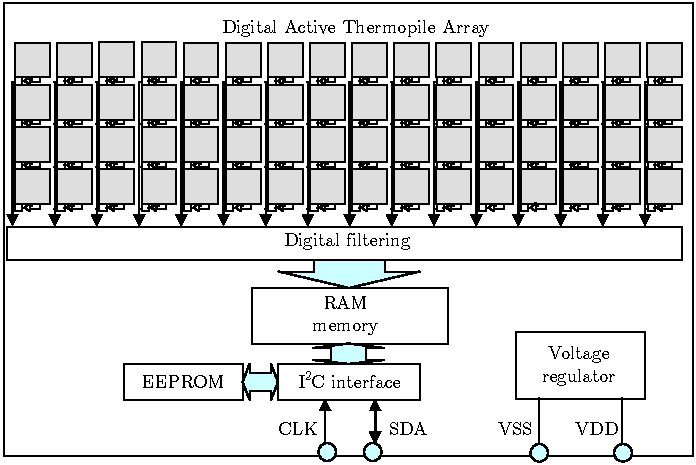
\includegraphics[width=0.8\textwidth]{../diagrams/mlx-block-diagram.pdf}
\caption{Block diagram for the \mlx taken from datasheet \cite{MLXDatasheet}}
\label{fig:exps:blockdia}
\end{figure}

\begin{figure}
\centering
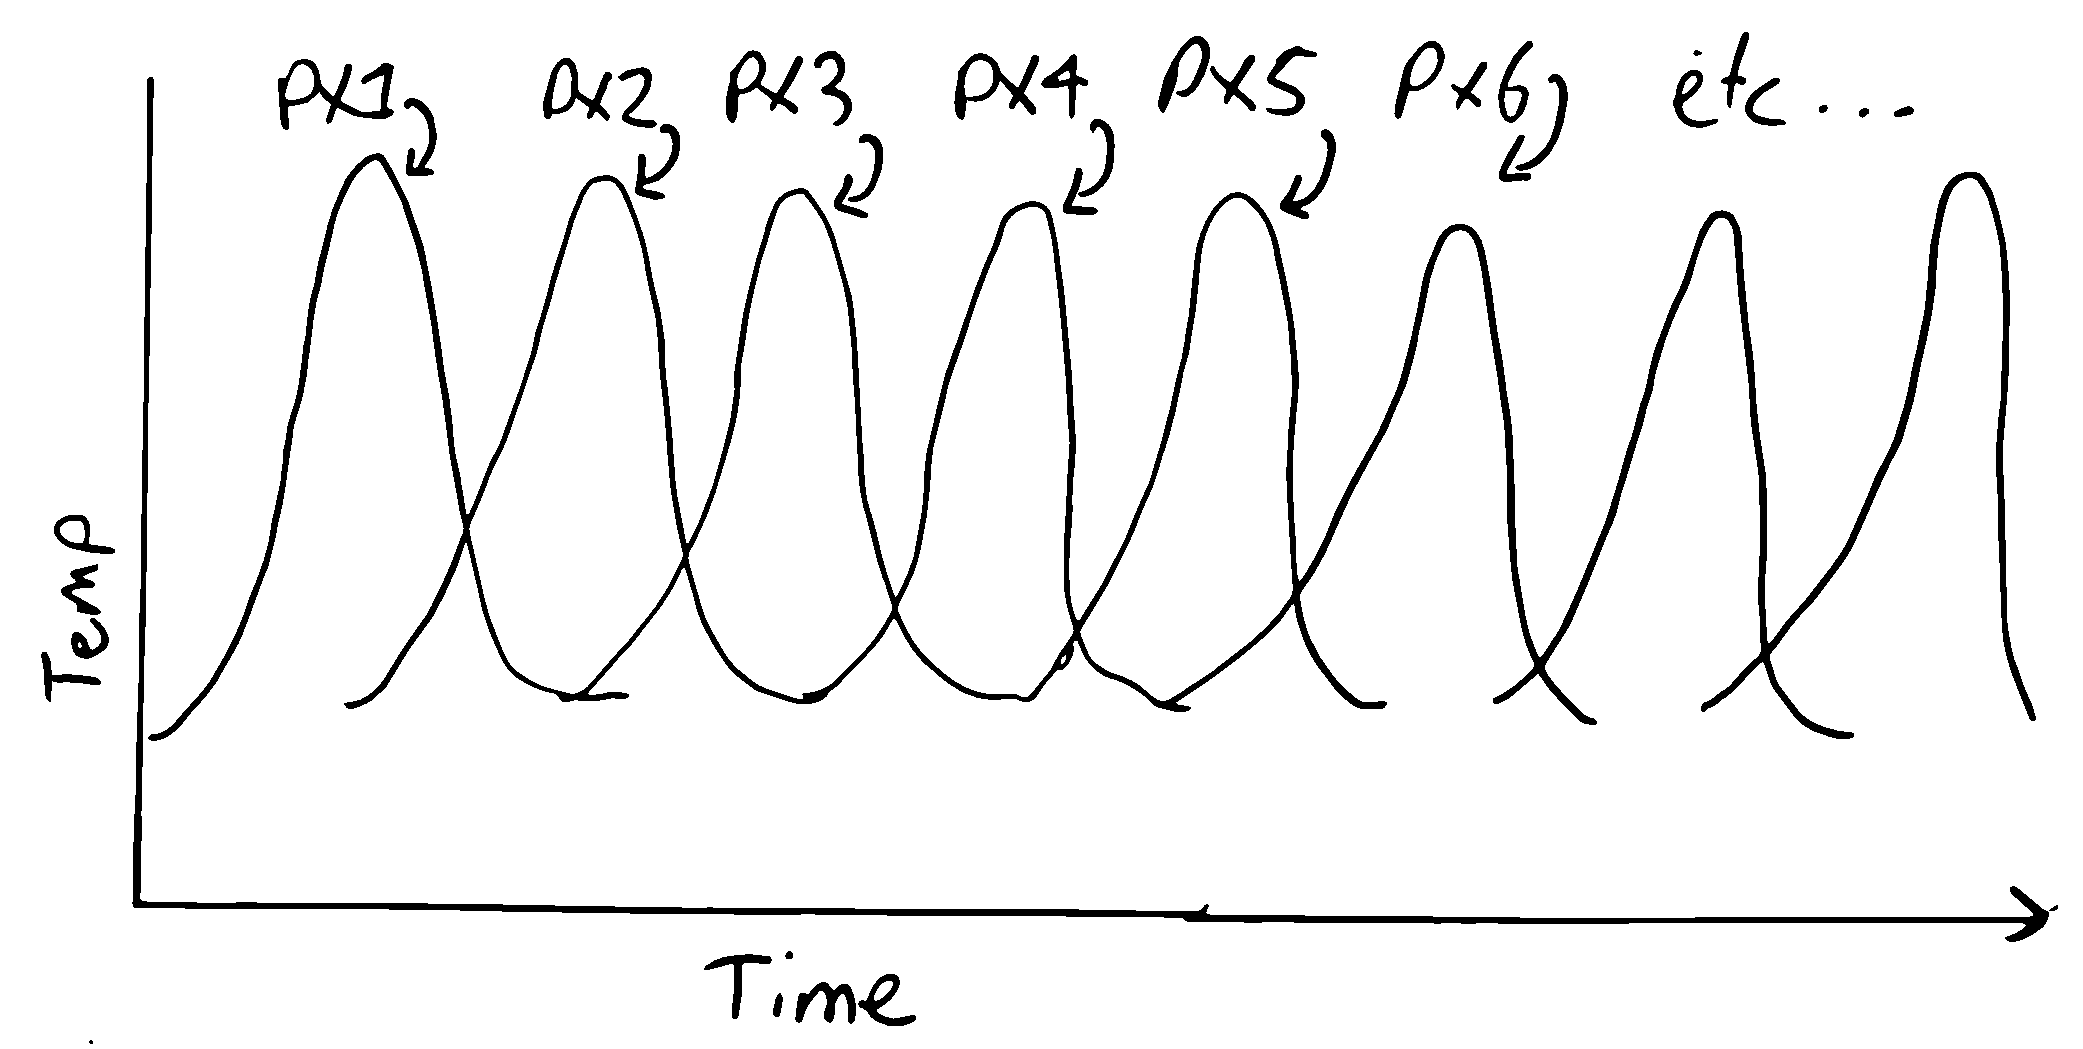
\includegraphics[width=\textwidth]{../diagrams/temp/motion.pdf}
\caption{Different \mlx pixel temperature values as hot object moves across row}
\label{fig:hotmotion}
\end{figure}

\begin{figure}
\centering
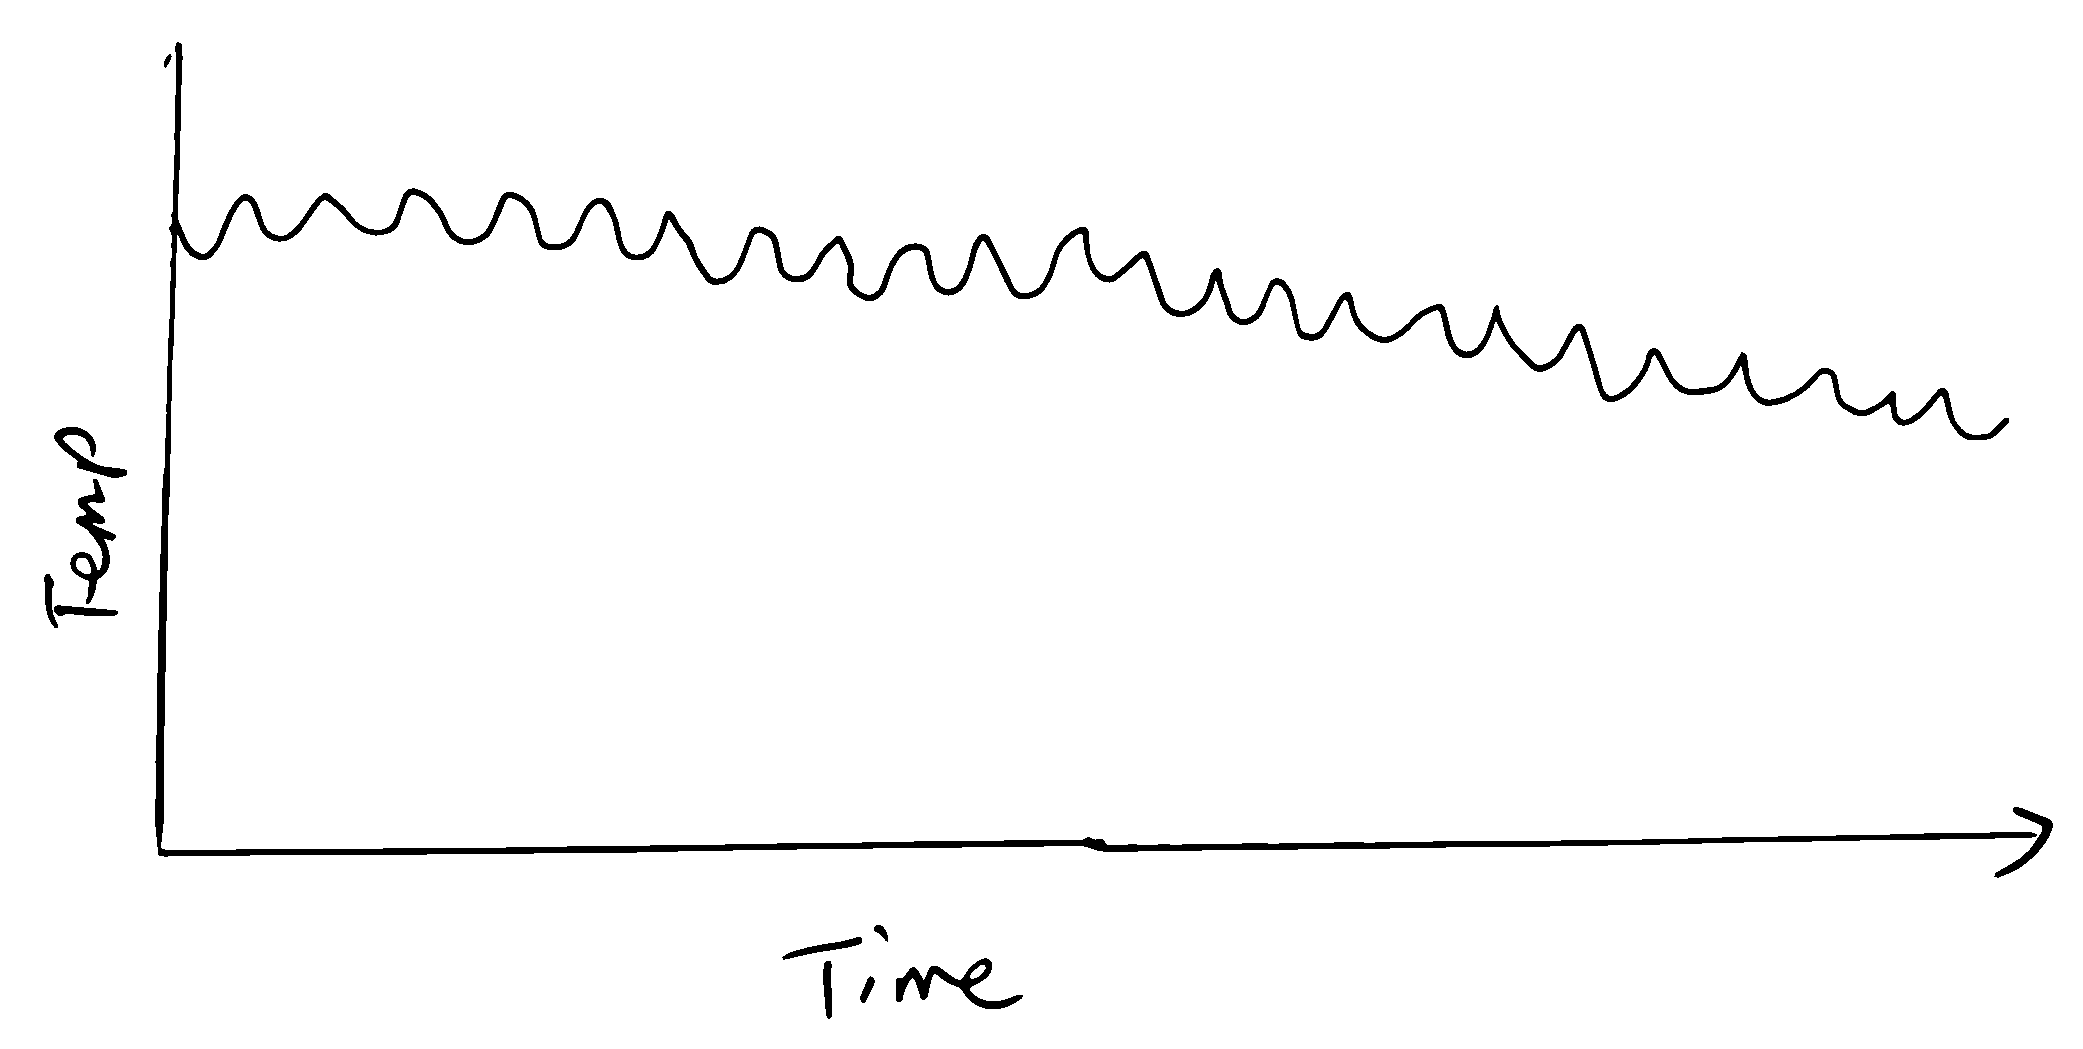
\includegraphics[width=\textwidth]{../diagrams/temp/cooldown.pdf}
\caption{Variation in temperature detected for hot object at 1Hz sampling ration}
\label{fig:cooldown}
\end{figure}
 
 \ifcsdef{mainfile}{}{\bibliography{../references/primary}}
\end{document}
